% !TEX TS-program = xelatex
% Command for running this example (needs latexmkrc file):
%    latexmk -bibtex -pdf main.tex

% این قالب با استفاده از کلاس kntu-thesis جهت نگارش گزارش پروژه، پایان‌نامه و رساله توسط محمدسینا اله‌کرم آماده سازی شده و از طریق لینک زیر در دسترس علاقه‌مندان قرار گرفته است.
%	https://github.com/msinamsina/kntu-thesis

%--------------------------------------------------------\right) \left( --------------------------------------
% اگر قصد نوشتن پروژه کارشناسی را دارید، در خط زیر به جای msc، کلمه bsc و اگر قصد نوشتن رساله دکترا را دارید، کلمه phd را قرار دهید. کلیه تنظیمات لازم، به طور خودکار، اعمال می‌شود.

% اگر مایلید پایان‌نامه شما دورو باشد به جای oneside در خط زیر از twoside استفاده کنید.

% برای حاشیه‌نویسی و کم کردن صفحات ابتدایی، گزینه draft را وارد و برای نسخه نهایی آن را حذف کنید.

% برای استفاده از قلم‌های سری IR Series گزینه irfonts را وارد و برای استفاده از قلم‌های X Series 2 آن را حذف کنید.



\documentclass[
twoside
% ,openany
,msc
,irfonts
% ,draft
]{./kntu-thesis}
\usepackage{placeins}
\usepackage{float}
\usepackage{matlab-prettifier}
\usepackage{pgfplots}

\usepackage{amsmath,amsfonts,amssymb}
\usepackage{longtable}
\usepackage{hyperref}
%\usepackage{geometry}
%\geometry{margin=1in}

% فایل commands.tex را مطالعه کنید؛ چون دستورات مربوط به فراخوانی بسته‌ها، فونت و دستورات خاص در این فایل قرار دارد.
% در این فایل، دستورها و تنظیمات مورد نیاز، آورده شده است.
%-------------------------------------------------------------------------------------------------------------------
% دستوراتی که پوشه پیش‌فرض زیرفایل‌های tex را مشخص می‌کند.
%\makeatletter
%\def\input@path{{./tex/}}
%\makeatother
% در ورژن جدید زی‌پرشین برای تایپ متن‌های ریاضی، این سه بسته، حتماً باید فراخوانی شود
\usepackage{amsthm,amssymb,amsmath}
% بسته‌ای برای تنطیم حاشیه‌های بالا، پایین، چپ و راست صفحه
\usepackage[a4paper, top=40mm, bottom=40mm, outer=25mm, inner=35mm]{geometry}
% بسته‌‌ای برای ظاهر شدن شکل‌ها و تعیین آدرس تصاویر
\usepackage[final]{graphicx}
\graphicspath{{./img/}}




% بسته‌های مورد نیاز برای نوشتن کدها، رنگ‌آمیزی آنها و تعیین پوشهٔ کدها
%%man ezafe kardam


\usepackage{diagbox}
\usepackage{multirow}
\usepackage[final]{listings}
\usepackage[usenames,dvipsnames,svgnames,table]{xcolor}
\lstset{inputpath=./code/}
\usepackage[notransparent]{svg}
\usepackage[final]{pdfpages}
\usepackage{tabularray}
\usepackage{booktabs, makecell, multirow, tabularx}
\usepackage{minted}

% بسته‌ای برای رسم کادر
\usepackage{framed} 
% بسته‌‌ای برای چاپ شدن خودکار تعداد صفحات در صفحه «معرفی پایان‌نامه»
\usepackage{lastpage}
% بسته‌ٔ لازم برای: ۱. تغییر شماره‌گذاری صفحات پیوست. ۲. تصحیح باگ آدرس وب حاوی '%' در مراجع
\usepackage{etoolbox}

%%%%%%%%%%%%%%%%%%%%%%%%%%%%%%%%%%%%
%%% دستورات وابسته به استیل مراجع:
%% اگر از استیل‌های natbib (plainnat-fa، asa-fa، chicago-fa) استفاده می‌کنید، خط زیر را فعال و بعدی‌اش را غیرفعال کنید.
%\usepackage{natbib}
%\newcommand{\citelatin}[1]{\cite{#1}\LTRfootnote{\citeauthor*{#1}}}
%\newcommand{\citeplatin}[1]{\citep{#1}\LTRfootnote{\citeauthor*{#1}}}


%% اگر از سایر استیل‌ها استفاده می‌کنید، خط بالا را غیرفعال و خط‌های زیر را فعال کنید.
\let\citep\cite
\let\citelatin\cite
\let\citeplatin\cite
%%%%%%%%%%%%
%% بررسی حالت پیش نویس
\usepackage{ifdraft}
\ifdraft
{%
	% بسته‌ٔ ایجاد لینک‌های رنگی با امکان جهش
	\usepackage[unicode=true,pagebackref=true,
colorlinks,linkcolor=blue,citecolor=blue,final]{hyperref}
	%\usepackage{todonotes}
	\usepackage[firstpage]{draftwatermark}
	\SetWatermarkText{\ \ \ \rl{پیش‌نویس}}
	\SetWatermarkScale{1.2}
}
{ 
	\usepackage[pagebackref=false]{hyperref}
	%\usepackage[disable]{todonotes} % final without TODOs
}

\usepackage[obeyDraft]{todonotes}
\setlength{\marginparwidth}{2cm}

%%%%%%%%%%%%
%%% تصحیح باگ: اگر در مراجع، آدرس وب حاوی '%' بوده و pagebackref فعال باشد، دستورات زیر باید بیایند:
%% برای استیل‌های natbib مثل plainnat-fa، asa-fa، chicago-fa
\makeatletter
\let\ORIG@BR@@lbibitem\BR@@lbibitem
\apptocmd\ORIG@BR@@lbibitem{\endgroup}{}{}
\def\BR@@lbibitem{\begingroup\catcode`\%=12 \ORIG@BR@@lbibitem}
\makeatother
%% برای سایر استیل‌ها
\makeatletter
\let\ORIG@BR@@bibitem\BR@@bibitem
\apptocmd\ORIG@BR@@bibitem{\endgroup}{}{}
\def\BR@@bibitem{\begingroup\catcode`\%=12 \ORIG@BR@@bibitem}
\makeatother
%%%%%%%%%%%%%%%%%%%%%%%%%%%%%%%%%%%%

% بسته‌ لازم برای تنظیم سربرگ‌ها
\usepackage{fancyhdr}
%\usepackage{enumitem}
\usepackage{setspace}
% بسته‌های لازم برای نوشتن الگوریتم
\usepackage{algorithm}
\usepackage{algorithmic}
% بسته‌های لازم برای رسم بهتر جداول
\usepackage{tabulary}
\usepackage{tabularx}
\usepackage{rotating}
% بسته‌های لازم برای رسم تنظیم بهتر شکل‌ها و زیرشکل‌ها
\usepackage[export]{adjustbox}
\usepackage{subfig}
\usepackage[subfigure]{tocloft}
% بسته‌ای برای رسم نمودارها و نیز صفحه مالکیت اثر
\usepackage{tikz}
% بسته‌ای برای ظاهر شدن «مراجع» و «نمایه» در فهرست مطالب
\usepackage[nottoc]{tocbibind}
% دستورات مربوط به ایجاد نمایه
\usepackage{makeidx}
\makeindex


% بسته‌ای برای افزودن تورفتگی به ابتدای اولین پاراگراف هر بخش
\usepackage{indentfirst}

% بسته زیر باگ ناشی از فراخوانی بسته‌های زیاد را برطرف می‌کند.
\usepackage{morewrites}
%%%%%%%%%%%%%%%%%%%%%%%%%%
%khodam
\RequirePackage{zref-perpage}
\zmakeperpage{footnote}

%%% بسته ایجاد واژه‌نامه با xindy
\usepackage[xindy,toc,acronym,nonumberlist=true]{glossaries}

% فراخوانی بسته زی‌پرشین (باید آخرین بسته باشد)
\usepackage[extrafootnotefeatures, localise=on, displaymathdigits=persian]{xepersian}
\paragraphfootnotes

\makeatletter
% تعریف قلم فارسی و انگلیسی و مکان قلم‌ها
\if@irfonts
\settextfont[Path={./font/}, BoldFont={IRLotusICEE_Bold.ttf}, BoldItalicFont={IRLotusICEE_BoldIranic.ttf}, ItalicFont={IRLotusICEE_Iranic.ttf},Scale=1.2]{IRLotusICEE.ttf}
% LiberationSerif or FreeSerif as free equivalents of Times New Roman
\setlatintextfont[Path={./font/}, BoldFont={LiberationSerif-Bold.ttf}, BoldItalicFont={LiberationSerif-BoldItalic.ttf}, ItalicFont={LiberationSerif-Italic.ttf},Scale=1]{LiberationSerif-Regular.ttf}
% چنانچه می‌خواهید اعداد در فرمول‌ها، انگلیسی باشد، خط زیر را غیرفعال کنید
% و گزینهٔ displaymathdigits=persian را از خط ۱۰۹ حذف کنید.
\setdigitfont[Path={./font/}, Scale=1.2]{IRLotusICEE.ttf}
% تعریف قلم‌های فارسی و انگلیسی اضافی برای استفاده در بعضی از قسمت‌های متن
\setiranicfont[Path={./font/}, Scale=1.3]{IRLotusICEE_Iranic.ttf}				% ایرانیک، خوابیده به چپ
\setmathsfdigitfont[Path={./font/}]{IRTitr.ttf}
%\defpersianfont\titlefont[Path={./font/}, Scale=1]{IRTitr.ttf}
\defpersianfont\titlefont[Path={./font/}, Scale=1]{IRLotusICEE.ttf}
% برای تعریف یک قلم خاص عنوان لاتین، خط بعد را فعال و ویرایش کنید و خط بعد از آن را غیرفعال کنید.
% \deflatinfont\latintitlefont[Scale=1]{LiberationSerif}
\font\latintitlefont=cmssbx10 scaled 2300 %cmssbx10 scaled 2300
\else
\settextfont{XB Niloofar}
\setlatintextfont{Junicode}
% چنانچه می‌خواهید اعداد در فرمول‌ها، انگلیسی باشد، خط زیر را غیرفعال کنید
% و گزینهٔ displaymathdigits=persian را از خط ۱۰۹ حذف کنید.
\setdigitfont{XB Niloofar}
% تعریف قلم‌های فارسی و انگلیسی اضافی برای استفاده در بعضی از قسمت‌های متن
% \setmathsfdigitfont{XB Titre}
\defpersianfont\titlefont{XB Titre}
\deflatinfont\latintitlefont[Scale=1.1]{Junicode}
\fi
\makeatother

% برای استفاده از قلم نستعلیق خط بعد را فعال کنید.
\defpersianfont\nast[Path={./font/}, Scale=2]{IranNastaliq}
% فونت‌های جدید را در این جا وارد کنید.
%\defpersianfont\newfont[Path={./font/}, Scale=2]{newfont}

%%%%%%%%%%%%%%%%%%%%%%%%%%
% راستچین شدن todonotes
\presetkeys{todonotes}{align=right,textdirection=righttoleft}{}
\makeatletter
\providecommand\@dotsep{5}
\def\listtodoname{فهرست کارهای باقیمانده}
\def\listoftodos{\noindent{\Large\vspace{10mm}\textbf{\listtodoname}}\@starttoc{tdo}}
\renewcommand{\@todonotes@MissingFigureText}{شکل}
\renewcommand{\@todonotes@MissingFigureUp}{شکل}
\renewcommand{\@todonotes@MissingFigureDown}{جاافتاده}
\makeatother
% دستوری برای حذف کلمه «چکیده»
% \renewcommand{\abstractname}{}
% دستوری برای حذف کلمه «abstract»
%\renewcommand{\latinabstract}{}
% دستوری برای تغییر نام کلمه «اثبات» به «برهان»
\renewcommand\proofname{\textbf{برهان}}
% دستوری برای تغییر نام کلمه «کتاب‌نامه» به «مراجع»
\renewcommand{\bibname}{مراجع}
% دستوری برای تعریف واژه‌نامه انگلیسی به فارسی
\newcommand\persiangloss[2]{#1\dotfill\lr{#2}\\}
% دستوری برای تعریف واژه‌نامه فارسی به انگلیسی 
\newcommand\englishgloss[2]{#2\dotfill\lr{#1}\\}
% تعریف دستور جدید «\پ» برای خلاصه‌نویسی جهت نوشتن عبارت «پروژه/پایان‌نامه/رساله»
\newcommand{\پ}{پروژه/پایان‌نامه/رساله }

%\newcommand\BackSlash{\char`\\}

%%%%%%%%%%%%%%%%%%%%%%%%%%
% \SepMark{-}

% تعریف و نحوه ظاهر شدن عنوان قضیه‌ها، تعریف‌ها، مثال‌ها و ...
\theoremstyle{definition}
\newtheorem{definition}{تعریف}[section]
\theoremstyle{theorem}
\newtheorem{theorem}[definition]{قضیه}
\newtheorem{lemma}[definition]{لم}
\newtheorem{proposition}[definition]{گزاره}
\newtheorem{corollary}[definition]{نتیجه}
\newtheorem{remark}[definition]{ملاحظه}
\theoremstyle{definition}
\newtheorem{example}[definition]{مثال}

%\renewcommand{\theequation}{\thechapter-\arabic{equation}}
%\def\bibname{مراجع}
\numberwithin{algorithm}{chapter}
\def\listalgorithmname{فهرست الگوریتم‌ها}
\def\listfigurename{فهرست تصاویر}
\def\listtablename{فهرست جداول}

% دستور های لازم برای تعریف ترجمهٔ دستورات الگوریتم
\makeatletter
\renewcommand{\algorithmicrequire}{\if@RTL\textbf{ورودی:}\else\textbf{Require:}\fi}
\renewcommand{\algorithmicensure}{\if@RTL\textbf{خروجی:}\else\textbf{Ensure:}\fi}
\renewcommand{\algorithmicend}{\if@RTL\textbf{پایان}\else\textbf{end}\fi}
\renewcommand{\algorithmicif}{\if@RTL\textbf{اگر}\else\textbf{if}\fi}
\renewcommand{\algorithmicthen}{\if@RTL\textbf{آنگاه}\else\textbf{then}\fi}
\renewcommand{\algorithmicelse}{\if@RTL\textbf{وگرنه}\else\textbf{else}\fi}
\renewcommand{\algorithmicfor}{\if@RTL\textbf{برای}\else\textbf{for}\fi}
\renewcommand{\algorithmicforall}{\if@RTL\textbf{برای هر}\else\textbf{for all}\fi}
\renewcommand{\algorithmicdo}{\if@RTL\textbf{انجام بده}\else\textbf{do}\fi}
\renewcommand{\algorithmicwhile}{\if@RTL\textbf{تا زمانی که}\else\textbf{while}\fi}
\renewcommand{\algorithmicloop}{\if@RTL\textbf{تکرار کن}\else\textbf{loop}\fi}
\renewcommand{\algorithmicrepeat}{\if@RTL\textbf{تکرار کن}\else\textbf{repeat}\fi}
\renewcommand{\algorithmicuntil}{\if@RTL\textbf{تا زمانی که}\else\textbf{until}\fi}
\renewcommand{\algorithmicprint}{\if@RTL\textbf{چاپ کن}\else\textbf{print}\fi}
\renewcommand{\algorithmicreturn}{\if@RTL\textbf{بازگردان}\else\textbf{return}\fi}
\renewcommand{\algorithmicand}{\if@RTL\textbf{و}\else\textbf{and}\fi}
\renewcommand{\algorithmicor}{\if@RTL\textbf{و یا}\else\textbf{or}\fi} % TODO add better translate
\renewcommand{\algorithmicxor}{\if@RTL\textbf{یا}\else\textbf{xor}\fi} % TODO add better translate
\renewcommand{\algorithmicnot}{\if@RTL\textbf{نقیض}\else\textbf{not}\fi}
\renewcommand{\algorithmicto}{\if@RTL\textbf{تا}\else\textbf{to}\fi}
\renewcommand{\algorithmicinputs}{\if@RTL\textbf{ورودی‌ها}\else\textbf{inputs}\fi}
\renewcommand{\algorithmicoutputs}{\if@RTL\textbf{خروجی‌ها}\else\textbf{outputs}\fi}
\renewcommand{\algorithmicglobals}{\if@RTL\textbf{متغیرهای عمومی}\else\textbf{globals}\fi}
\renewcommand{\algorithmicbody}{\if@RTL\textbf{انجام بده}\else\textbf{do}\fi}
\renewcommand{\algorithmictrue}{\if@RTL\textbf{درست}\else\textbf{true}\fi}
\renewcommand{\algorithmicfalse}{\if@RTL\textbf{نادرست}\else\textbf{false}\fi}
\renewcommand{\algorithmicendif}{\algorithmicend\textbf{ شرط }\algorithmicif}
\renewcommand{\algorithmicendfor}{\algorithmicend\textbf{ حلقهٔ }\algorithmicfor}
\renewcommand{\algorithmicendwhile}{\algorithmicend\textbf{ حلقهٔ }\algorithmicwhile}
\renewcommand{\algorithmicendloop}{\algorithmicend\textbf{ حلقهٔ }\algorithmicloop}
\renewcommand{\algorithmiccomment}[1]{\{{\itshape #1}\}}
\makeatletter

%%%%%%%%%%%%%%%%%%%%%%%%%%%%
%%% دستورهایی برای سفارشی کردن سربرگ صفحات:
%\newcommand{\SetHeader}[1]{
% دستور زیر معادل با گزینه twoside است.
%\csname@twosidetrue\endcsname
\pagestyle{fancy}
%% دستورات زیر سبک صفحات fancy را تغییر می‌دهد:
% O=Odd, E=Even, L=Left, R=Right
% در صورت oneside بودن، عنوان فصل، سمت چپ ظاهر می‌شود.
\fancyhead{}
\fancyhead[OR]{\small\leftmark}
\fancyhead[ER]{\small\leftmark}
\fancyhead[OL,EL]{\thepage}
\fancyfoot{} % حذف محتوای پیش‌فرض پانویس
%\fancyhead[ER]{\small\rightmark}
%\fancyhead[OR]{\footnotesize}
%\fancyhead[EL]{\footnotesize\rightmark}
\renewcommand{\headrulewidth}{0.75pt}
% شکل‌دهی شماره و عنوان فصل در سربرگ
\renewcommand{\chaptermark}[1]{\markboth{\@chapapp~\thechapter:\ #1}{}}
\makeatletter
%\renewcommand{\rightmark}[1]{\@title}
%\makeatother
%}
% شکل‌دهی سربرگ در صفحات اولیه هر فصل
\patchcmd{\chapter}{\thispagestyle{plain}}{\thispagestyle{empty}}{}{}
%%%%%%%%%%%%%%%%%%%%%%%%%%%%
%\def\MATtextbaseline{1.5}
%\renewcommand{\baselinestretch}{\MATtextbaseline}
\doublespacing
%%%%%%%%%%%%%%%%%%%%%%%%%%%%%
% دستوراتی برای اضافه کردن کلمه «فصل» در فهرست مطالب

\newlength\mylenprt
\newlength\mylenchp
\newlength\mylenapp

\renewcommand\cftpartpresnum{\partname~}
\renewcommand\cftchappresnum{\chaptername~}
\renewcommand\cftchapaftersnum{:}

\settowidth\mylenprt{\cftpartfont\cftpartpresnum\cftpartaftersnum}
\settowidth\mylenchp{\cftchapfont\cftchappresnum\cftchapaftersnum}
\settowidth\mylenapp{\cftchapfont\appendixname~\cftchapaftersnum}
\addtolength\mylenprt{\cftpartnumwidth}
\addtolength\mylenchp{\cftchapnumwidth}
\addtolength\mylenapp{\cftchapnumwidth}

\setlength\cftpartnumwidth{\mylenprt}
\setlength\cftchapnumwidth{\mylenchp}	

\makeatletter
{\def\thebibliography#1{\chapter*{\refname\@mkboth
   {\uppercase{\refname}}{\uppercase{\refname}}}\list
   {[\arabic{enumi}]}{\settowidth\labelwidth{[#1]}
   \rightmargin\labelwidth
   \advance\rightmargin\labelsep
   \advance\rightmargin\bibindent
   \itemindent -\bibindent

   \listparindent \itemindent
   \parsep \z@
   \usecounter{enumi}}
   \def\newblock{}
   \sloppy
   \sfcode`\.=1000\relax}}
   
%اگر مایلید در شماره گذاری حرفی و ابجد به جای آ از الف استفاده شود دستورات زیر را فعال کنید.   
%\def\@Abjad#1{%
%  \ifcase#1\or الف\or ب\or ج\or د%
%           \or هـ\or و\or ز\or ح\or ط%
%           \or ی\or ک\or ل\or م\or ن%
%           \or س\or ع\or ف\or ص%
%           \or ق\or ر\or ش\or ت\or ث%
%            \or خ\or ذ\or ض\or ظ\or غ%
%            \else\@ctrerr\fi}
%
% \def\abj@num@i#1{%
%   \ifcase#1\or الف\or ب\or ج\or د%
%            \or هـ‍\or و\or ز\or ح\or ط\fi

%   \ifnum#1=\z@\abjad@zero\fi}   
%  
%   \def\@harfi#1{\ifcase#1\or الف\or ب\or پ\or ت\or ث\or

% ج\or چ\or ح\or خ\or د\or ذ\or ر\or ز\or ژ\or س\or ش\or ص\or ض\or ط\or ظ\or ع\or غ\or

% ف\or ق\or ک\or گ\or ل\or م\or ن\or و\or ه\or ی\else\@ctrerr\fi}

%
\makeatother

%%% امکان درج کد در سند
% در این قسمت رنگ، قلم و قالب‌بندی قسمت‌های مختلف یک کد تعیین می‌شود. 
\lstdefinestyle{myStyle}{
	basicstyle=\ttfamily, % whole listing /w verbatim font
	keywordstyle=\color{blue}\bfseries, % bold black keywords
	identifierstyle=, % nothing happens
	commentstyle=\color{LimeGreen}, % green comments
	stringstyle=\ttfamily\color{red}, % red typewriter font for strings
	showstringspaces=false % no special string spaces
	breaklines=true,
	breakatwhitespace=false,
	numbers=right, % line number formats
	numberstyle=\footnotesize\lr,
	numbersep=-10pt,
	frame=single,
	captionpos=b,
	captiondirection=RTL
}
\lstset{style=myStyle} % command to set default style
\def\lstlistingname{\rl{برنامهٔ}}
\def\lstlistlistingname{\rl{فهرست برنامه‌ها}}


% for numbering subsubsections
\setcounter{secnumdepth}{3}
%to include subsubsections in the table of contents
\setcounter{tocdepth}{3}

\makeatletter
\renewcommand{\p@subfigure}{\thefigure.}
\makeatother


% مشخصات پایان‌نامه را در فایلهای faTitle و enTitle وارد نمایید.
% !TeX root=../main.tex
% در این فایل، عنوان پایان‌نامه، مشخصات خود، متن تقدیمی‌، ستایش، سپاس‌گزاری و چکیده پایان‌نامه را به فارسی، وارد کنید.
% توجه داشته باشید که جدول حاوی مشخصات پروژه/پایان‌نامه/رساله و همچنین، مشخصات داخل آن، به طور خودکار، درج می‌شود.
%%%%%%%%%%%%%%%%%%%%%%%%%%%%%%%%%%%%
% دانشگاه خود را وارد کنید
\university{دانشگاه خواجه نصیرالدین طوسی}
% پردیس دانشگاهی خود را اگر نیاز است وارد کنید (مثال: فنی، علوم پایه، علوم انسانی و ...)
\college{...}
% دانشکده، آموزشکده و یا پژوهشکده  خود را وارد کنید
\faculty{دانشکده برق}
% گروه آموزشی خود را وارد کنید (در صورت نیاز)
\department{گروه مکاترونیک}
% رشته تحصیلی خود را وارد کنید
\subject{رشته مهندسی مکاترونیک}
% در صورت داشتن گرایش، خط زیر را از حالت کامت خارج نموده و گرایش خود را وارد کنید
% \field{گرابش}
% عنوان پایان‌نامه را وارد کنید
\title{ تمرین درس یادگیری ماشین }
% نام استاد(ان) راهنما را وارد کنید
%\firstsupervisor{دکتر مهدی علیاری شوره دلی}
%\firstsupervisorrank{دانشیار}
%\secondsupervisor{دکتر اسماعیل نجفی}
%\secondsupervisorrank{استادیار}
% نام استاد(دان) مشاور را وارد کنید. چنانچه استاد مشاور ندارید، دستورات پایین را غیرفعال کنید.
%\firstadvisor{دکتر مشاور اول}
%\firstadvisorrank{استادیار}
%\secondadvisor{دکتر مشاور دوم}
% نام داوران داخلی و خارجی خود را وارد نمایید.
%\internaljudge{دکتر داور داخلی}
%\internaljudgerank{دانشیار}
%\externaljudge{دکتر داور خارجی}
%\externaljudgerank{دانشیار}
%\externaljudgeuniversity{دانشگاه داور خارجی}
% نام نماینده کمیته تحصیلات تکمیلی در دانشکده \ گروه
%\graduatedeputy{دکتر نماینده}
%\graduatedeputyrank{دانشیار}
% نام دانشجو را وارد کنید
\name{علیرضا}
% نام خانوادگی دانشجو را وارد کنید
\surname{امیری}
% شماره دانشجویی دانشجو را وارد کنید
\studentID{40202414}
% تاریخ پایان‌نامه را وارد کنید
\thesisdate{اسفند 1403}
% به صورت پیش‌فرض برای پایان‌نامه‌های کارشناسی تا دکترا به ترتیب از عبارات «پروژه»، «پایان‌نامه» و «رساله» استفاده می‌شود؛ اگر  نمی‌پسندید هر عنوانی را که مایلید در دستور زیر قرار داده و آنرا از حالت توضیح خارج کنید.
\projectLabel{تمرین یادگیری ماشین}

% به صورت پیش‌فرض برای عناوین مقاطع تحصیلی کارشناسی تا دکترا به ترتیب از عبارت «کارشناسی»، «کارشناسی ارشد» و «دکتری» استفاده می‌شود؛ اگر نمی‌پسندید هر عنوانی را که مایلید در دستور زیر قرار داده و آنرا از حالت توضیح خارج کنید.
%\degree{}
%%%%%%%%%%%%%%%%%%%%%%%%%%%%%%%%%%%%%%%%%%%%%%%%%%%%
%% پایان‌نامه خود را تقدیم کنید! %%
%\dedication
%{
%{\Large تقدیم به:}\\
%\begin{flushleft}{
%	\huge
%به آنان که با علم خود زندگی آزاد می‌سازند\\
%	\vspace{7mm}
%}
%\end{flushleft}
%}
%% متن قدردانی %%
%% این متن را به سلیقه‌ی خود تعییر دهید
%\acknowledgement{
%اکنون که به یاری پروردگار و یاری و راهنمایی اساتید بزرگ موفق به پایان این رساله شده‌ام وظیفه خود دانشته که نهایت سپاسگزاری را از تمامی عزیزانی که در این راه به من کمک کرده‌اند را به عمل آورم:
%در آغاز از استاد بزرگ و دانشمند جناب آقای/سرکار خانم …. که راهنمایی این پایانامه را به عهده داشته‌اند کمال تشکر را دارم.
%از جناب آقایان/ خانم‌ها …. که اساتید مشاور این پایانامه بوده‌اند نیز قدردانی می‌نمایم.
%از داوران گرامی … که زحمت داوری و تصحیح این پایانامه را به عهده داشتند کمال سپاس را دارم.
%خالصانه از تمامی اساتید و معلمان و مدرسانی که در مقاطع مختلف تحصیلی به من علم آموخته و مرا از سرچشمه دانایی سیراب کرده‌اند متشکرم.
%از کلیه هم دانشگاهیان و همراهان عزیز، دوستان خوبم خانم‌ها و آقایان …. نهایت سپاس را دارم.
%
%و در پایان این پایان‌نامه را تقدیم می‌کنم به …. که با حضورش و همراهی اش همیشه راه را به من نشان داده و مرا در این راه استوار و ثابت قدم نموده است.
%}
%%%%%%%%%%%%%%%%%%%%%%%%%%%%%%%%%%%%
%چکیده پایان‌نامه را وارد کنید
%\fa-abstract{

%}
% کلمات کلیدی پایان‌نامه را وارد کنید
%\keywords{شناوری مغناطیسی، آرایه هالباخ، کنترلر مبتنی بر پیش‌بینی مدل}




% انتهای وارد کردن فیلد‌ها
%%%%%%%%%%%%%%%%%%%%%%%%%%%%%%%%%%%%%%%%%%%%%%%%%%%%%%

% مشخصات انگلیسی پایان‌نامه
% !TeX root=../main.tex
% در این فایل، عنوان پایان‌نامه، مشخصات خود و چکیده پایان‌نامه را به انگلیسی، وارد کنید.

%%%%%%%%%%%%%%%%%%%%%%%%%%%%%%%%%%%%
\latinuniversity{K. N. Toosi University of Technology}
\latincollege{...}
\latinfaculty{Faculty of Electrical Engineering}
\latindepartment{Mechatronics Group}
\latinsubject{Mechatronics Engineering}
%\latinfield{field}
\latintitle{Analyzing Design and Implementation methods of Magnetically Levitated Planar Motors}
\firstlatinsupervisor{Mahdi Aliyari Shooredeli}
\secondlatinsupervisor{Esmaeil Najafi}
%\firstlatinadvisor{First Advisor}
%\secondlatinadvisor{Second Advisor}
\latinname{Alireza}
\latinsurname{Amiri}
\latinthesisdate{Summer 2024}
\latinkeywords{Magnetic levitation, Planar motors, Halbach array, Model Predicting Control, Contactless operation}
\en-abstract{
Magnetic levitation planar motors (MLPM) offer precise, contactless motion, making them ideal for applications requiring high-accuracy positioning, such as in manufacturing, automation, and robotics. However, designing and optimizing MLPM systems involves overcoming challenges related to system architecture, magnet configuration, control strategies, and modeling techniques, all of which significantly impact the performance and efficiency of these devices.
This study examines four key aspects of MLPM systems. First, the architecture of the system is analyzed, with a focus on the choice between moving-coil and fixed-coil designs. The findings suggest that fixed-coil designs, where the magnets are placed on the moving component, reduce physical constraints such as electrical connections and improve cooling efficiency, making them more suitable for real-world applications. Second, the design of permanent magnets is explored, specifically comparing disc magnets with Halbach arrays. Halbach arrays, especially in two-dimensional configurations, are found to provide stronger, more concentrated magnetic fields with greater control precision, outperforming traditional magnet designs.
In the third aspect, control strategies are evaluated, with classical PID controllers being compared to more advanced techniques like Model Predictive Control (MPC) and AI-based methods such as Gated Recurrent Units (GRU). While PID controllers are effective for basic applications, advanced control techniques leveraging system dynamics and machine learning demonstrate improved stability and reduced error in controlling MLPM systems.
Finally, the study explores modeling approaches, contrasting analytical methods with numerical techniques like finite element modeling (FEM). The analysis reveals that while analytical models provide a foundational understanding, numerical simulations, particularly FEM, offer greater accuracy and flexibility in designing and validating complex MLPM systems.
In conclusion, this research highlights the advantages of using fixed-coil architecture, Halbach magnet arrays, advanced control strategies, and numerical modeling techniques for optimizing MLPM performance, paving the way for their broader application in precision-driven industries.
}


% تنظیمات و تعاریف واژه‌نامه و اختصارات در صورتی که نمی‌خواهید واژه‌نامه‌ها و اختصارات نمایش داده شوند سه خط زیر را کامنت نمایید.
%\input{./tex/glossaries-settings}
%\input{./tex/words}
%\input{./tex/acronyms.tex}



\begin{document}

\pagenumbering{adadi} % یک، دو، ...
% ابتدای درج صفحات مختلف
%\coverPage
% بررسی حالت پیش‌نویس
\ifoptiondraft{}{% 
    \titlePage
    %\besmPage
% چنانچه مایل به چاپ صفحات «تقدیم»، «نیایش» و «سپاس‌گزاری» در خروجی نیستید، خط‌های زیر را با گذاشتن ٪  در ابتدای آنها غیرفعال کنید.
%    \taghdimPage
 %  \davaranPage
%%%%%%%%%%%%%%%%%%%%%%%%%%%
%    \esalatPage
%    \mojavezPage
%    \ghadrdaniPage
} % end ifoptiondraft
%\abstractPage
% شروع درج فهرست‌ها

%\cleardoublepage
\clearpage
\pagenumbering{harfi} % آ، ب، ...
%\tableofcontents \clearpage
% بررسی حالت پیش‌نویس برای بقیه فهرست‌ها
\ifoptiondraft{
 %   \listoftodos
}{%

% % Redefining the name of the list of figures to "فهرست شکل‌ها"
% \renewcommand{\listfigurename}{فهرست شکل‌ها}

% % Redefining the name of the list of tables to "فهرست جدول‌ها"
% \renewcommand{\listtablename}{فهرست جدول‌ها}

%\listoffigures \clearpage
%\listoftables  \clearpage
% فهرست الگوریتم‌ها: اگر نیازی به ایجاد فهرست الگوریتم‌ها ندارید دو خط زیر را کامنت کنید
%\addcontentsline{toc}{chapter}{\listalgorithmname}
%\listofalgorithms \clearpage
% فهرست برنامه‌ها: اگر نیازی به ایجاد فهرست برنامه‌ها ندارید دو خط زیر را کامنت کنید
%\addcontentsline{toc}{chapter}{\lstlistlistingname}
%\lstlistoflistings \clearpage
% فهرست اختصارات: اگر نیازی به ایجاد فهرستاختصارات ندارید خط زیر را کامنت کنید
%\printacronyms
} % end ifoptiondraft


\pagestyle{fancy}
\pagenumbering{arabic} % 1, 2, ...

% !TeX root=../main.tex

\chapter{پاسخ سوالات سری اول}

\href{https://drive.google.com/drive/folders/1BMXUcHZQBMV6n8P9XX5LD0nV40Ff3FDP?usp=drive_link}{Google Drive Folder}

% دستور زیر باعث عدم‌نمایش شماره صفحه در اولین صفحهٔ این فصل می‌شود.
%\thispagestyle{empty}
\section{ پاسخ سوال 1}
\subsection{قسمت اول، بخش الف}
برای محاسبه ابعاد ماتریس ها پس از ضرب دو ماتریس در یک دیگر، در صورتی که ابعاد ماتریس اول X برابر با $m * n$ و ابعاد ماتریس دوم Y برابر $u * v$ باشد، می توانیم از رابطه ی زیر استفاده می کنیم. 
\[
X_{m \times n} \cdot Y_{u \times v} = Z_{m \times v}
\]
برای ماتریس های داده شده داریم:
\[
size(A) = 2*3 , size(B) = 4*2
\]
در نتیجه، سایز ماتریس های داده شده برابر خواهد بود با:
\[
size(B \times A) = 4*3 
\]
\[
size(B^{T}) = 2*4 
\]
\[
size(B^{T} \times A) = Null 
\]
\[
size(A^{T} \times B) = Null 
\]
ماتریس هایی که قابل ضرب شدن نیستند، به دلیل تناقض در ابعاد ماتریس ها و عدم همخوانی تعداد ستون های ماتریس اول با تعداد سطر های ماتریس دوم می باشد.

\subsection{قسمت اول، بخش ب}
ماتریس های مطرح شده در بخش قبل به صورت زیر خواهند بود.
\[
BA =
\begin{bmatrix}
	b_{11} & b_{12} \\
	b_{21} & b_{22} \\
	b_{31} & b_{32} \\
	b_{41} & b_{42}
\end{bmatrix}
\begin{bmatrix}
	a_{11} & a_{12} & a_{13} \\
	a_{21} & a_{22} & a_{23}
\end{bmatrix}
=
\begin{bmatrix}
	b_{11} a_{11} + b_{12} a_{21} & b_{11} a_{12} + b_{12} a_{22} & b_{11} a_{13} + b_{12} a_{23} \\
	b_{21} a_{11} + b_{22} a_{21} & b_{21} a_{12} + b_{22} a_{22} & b_{21} a_{13} + b_{22} a_{23} \\
	b_{31} a_{11} + b_{32} a_{21} & b_{31} a_{12} + b_{32} a_{22} & b_{31} a_{13} + b_{32} a_{23} \\
	b_{41} a_{11} + b_{42} a_{21} & b_{41} a_{12} + b_{42} a_{22} & b_{41} a_{13} + b_{42} a_{23}
\end{bmatrix}
\]

\[
B^T =
\begin{bmatrix}
	b_{11} & b_{21} & b_{31} & b_{41} \\
	b_{12} & b_{22} & b_{32} & b_{42}
\end{bmatrix}
\]


\subsection{قسمت دوم، بخش اول}
با در نظر داشتن ابعاد ماتریس x برابر با $1*2$ و ابعاد ماتریس $\theta$ برابر با $2*1$، ابعاد ماتریس $x*\theta$ برابر با $1*1$ خواهد بود.
با افزایش تعداد نمونه ها در سطر های جدیدی برای ماتریس 
\textbf{X}،
ابعاد ماتریس 
$\textbf{X} \times \theta$
برابر 
$n*1$
خواهد بود.
\subsection{قسمت دوم، بخش دوم}
\[
X\theta - \vec{y} =
\begin{bmatrix}
	x^{(1)T}\theta \\
	\vdots \\
	x^{(n)T}\theta
\end{bmatrix}
-
\begin{bmatrix}
	y^{(1)} \\
	\vdots \\
	y^{(n)}
\end{bmatrix}
=
\begin{bmatrix}
	h_\theta(x^{(1)}) - y^{(1)} \\
	\vdots \\
	h_\theta(x^{(n)}) - y^{(n)}
\end{bmatrix}.
\]

آنگاه با در نظر داشتن آنکه \( z \), خواهیم داشت \( z^T z = \sum_i z_i^2 \):

\[
\frac{1}{2}(X\theta - \vec{y})^T(X\theta - \vec{y}) = \frac{1}{2}\sum_{i=1}^{n}(h_\theta(x^{(i)}) - y^{(i)})^2 = J(\theta)
\]

سپس، برای کاهش مقدار \( J \) مشتق آن را نسبت به \( \theta \) به دست می آوریم.

\[
\nabla_\theta J(\theta) = \nabla_\theta \frac{1}{2}(X\theta - \vec{y})^T(X\theta - \vec{y})
\]

\[
= \frac{1}{2}\nabla_\theta \left( (X\theta)^T X\theta - (X\theta)^T\vec{y} - \vec{y}^T (X\theta) + \vec{y}^T\vec{y} \right)
\]

\[
= \frac{1}{2}\nabla_\theta \left( \theta^T (X^T X)\theta - \vec{y}^T (X\theta) - \vec{y}^T (X\theta) \right)
\]

\[
= \frac{1}{2}\nabla_\theta \left( \theta^T (X^T X)\theta - 2(X^T\vec{y})^T\theta \right)
\]

\[
= \frac{1}{2} \left( 2X^T X\theta - 2X^T\vec{y} \right)
\]

\[
= X^T X\theta - X^T\vec{y}
\]

\section{پاسخ سوال 2}
\subsection{پرده اول}
با در اختیار داشتن فرمول احتمال بیز به صورت زیر خواهیم داشت:
\[
P(+) = P(+ \cap \text{sick}) + P(+ \cap \text{$not sick$})
\]
در این رابطه، احتمال کل مثبت بودن نتیجه آزمایش در حالت مریض بودن یا نبودن محاسبه می شود. 
\[
P(+) = P(+ | \text{sick}) P(\text{sick}) + P(+ | \text{$not sick$}) P(\text{$not sick$})
\]
با جایگذاری مقادیر عددی خواهیم داشت:
\[
P(+) = \frac{99}{100} \cdot 10^{-4} + \frac{1}{100} \cdot \frac{9999}{10000} = 0.0010098
\]
حال با استفاده از فرمول بیز خواهیم داشت:
\[
P(\text{sick} | +) = \frac{P(+ | \text{sick}) P(\text{sick})}{P(+)}
\]
\[
P(\text{sick} | +) = \frac{0.000099}{0.0010098} \approx 0.0980392
\]

\subsection{پرده دوم}
در این پرده، به محاسبه ی احتمال بیمار بودن علی در صورتی که پاسخ هر دو تست مثبت باشند خواهیم پرداخت.

\[
P(\text{sick} | ++) = ?
\]
مجددا با استفاده از قانون احتمال کل خواهیم داشت:
\[
P(++) = P(++ | \text{sick}) P(\text{sick}) + P(++ | \text{$not sick$}) P(\text{$not sick$})
\]
که با جایگذاری مقادیر احتمال ها خواهیم داشت:
\[
P(++) = \frac{99}{100} \cdot \frac{9999}{10000} \cdot 10^{-4} + \frac{1}{100} \cdot \frac{1}{10000} \cdot \frac{9999}{10000}
\]
\[
= 0.00009899 + 0.00000000999
\]
\[
= 0.000099999 \approx 0.0001
\]
در پایان، با استفاده از رابطه ی بیز چنین به دست می آوریم:
\[
P(\text{sick} | ++) = \frac{P(++ | \text{sick}) P(\text{sick})}{P(++)}
\]
در اینجا خواهیم داشت:
\[
P(\text{sick} | ++) = \frac{P(++ | \text{sick}) P(\text{sick})}{P(++)}
\]
و با جایگذاری مقادیر به دست آمده در رابطه ی بالا خواهیم داشت:
\[
= \frac{0.989901 \times 10^{-4}}{0.0001}
\]
\[
= 0.9899
\]
\[
P(\text{sick} | ++) \approx 0.9899
\]
\subsection{پرده سوم}
\[
P(\text{sick} | ++-) = \frac{P(++- | \text{sick}) P(\text{sick})}{P(++-)}
\]
ابتدا به محاسبه ی  \( P(++-) \) می پردازیم:
\[
P(++-) = P(++- | \text{sick}) P(\text{sick}) + P(++- | \text{$not sick$}) P(\text{$not sick$})
\]
با جایگذاری مقادیر به دست می آوریم:
\[
= (0.99 \cdot 0.9999 \cdot 0.000001) \cdot 10^{-4} + (0.01 \cdot 0.0001 \cdot \frac{999999}{1000000}) \cdot \frac{9999}{10000}
\]
\[
= 0.000000989901 \cdot 0.0001 + 0.000000999 \cdot 0.9999
\]
\[
\approx 0.000000998
\]
\[
P(\text{sick} | ++-) = \frac{0.000000989901 \cdot 10^{-4}}{0.000000998}
\]
\[
\approx 9.918847 \cdot 10^{-5}
\]
\section{پاسخ سوال 3، قسمت اول}
\subsection{بخش الف، دریافت داده}
\subsubsection{1}
برای این قسمت، فایل 149 از مجموعه داده های قرار داده شده در سایت توسط نرم افزار های مدیریت دانلود، دانلود می شود. فرمت این فایل $.mat$ است.
برای استفاده از این فایل، ابتدا آن را در فضای ابری درایو ذخیره کرده و با ایجاد دسترسی برای آن فایل و استفاده از دستور gdown، آن را در محیط گوگل کولب وارد می کنیم. 
در ادامه، با استفاده از دستور loadmat از پکیج scipy.io، می توانیم دیتا را در یک متغیر ذخیره می کنیم. 
\begin{minted}{python}
!pip install --upgrade --no-cache-dir gdown

!gdown 1zKj4N5nFFKK1u9AhzlqJLvsw-xRC0kz_

from scipy.io import loadmat
file_path = '/content/149.mat'
mat_data = loadmat(file_path)
\end{minted}
\subsubsection{2}
پس از ذخیره سازی فایل، در متغیر بالا، می توانیم به جستجو درباره ویژگی های آن بپردازیم. با استفاده از دستور type مشاهده می کنیم که متغیر ذخیره شده از جنس dictionary است.
یک دیکشنری متشکل از بخش های زیر است:
\begin{enumerate}
	\item \textbf{Key} 
	کلید، مشخصه ای منحصر به فرد به ازای هر مقدار در دیکشنری است.
	\item \textbf{value}
	حاوی مقدار عددی مرتبط با یک key است و می تواند مقادیر تکراری داشته باشد.
	\item \textbf{item}
	به زوج key و value متناظر آن یک item گفته می شود و با علامت $:$ با یکدیگر مرتبط می شوند.
\end{enumerate}
\subsubsection{3}
در این بخش، با مشاهده ی کلید های موجود در دیکشنری سیستم خواهیم دید که این مجموعه داده توسط کلید های زیر تعریف شده اند.
\_\_header\_\_, \_\_version\_\_, \_\_globals\_\_, X149\_DE\_time, X149\_FE\_time, X149RPM
و از میان این مقادیر، دو سیگنال $X149\_DE\_time$ و $X149\_FE\_time$ حاوی سیگنال های اطلاعات هستند. در این بخش سیگنال $X149\_DE\_time$ انتخاب و در متغیری ذحیره می شود.
\subsection{بخش ب، نمایش سیگنال}
برای نمایش سیگنال انتخاب شده، لازم از کتابخانه ی Matplotlib استفاده شود. برای نمایش سیگنال، علاوه بر در اختیار داشتن خود سیگنال باید مقدار محور افقی که در این سوال برابر با زمان خواسته شده است نیز محاسبه شود. با در نظر داشتن فرکانس نمونه برداری برابر با 480000، مقادیر محور افقی با استفاده از دستور linspace در پکیج numpy ایجاد می شود. با تنظیم ابعاد نمودار مورد نظر با استفاده از دستور figure و تعیین ابعاد نمودار، می توانیم نمودار مورد نظر را نمایش دهیم.
\begin{minted}{python}
import numpy as np
import matplotlib.pyplot as plt

fs = 48000 #KHz
time = np.linspace(0, len(DE_time)/fs , len(DE_time))

plt.figure(figsize=(30,5))
plt.plot(time, DE_time)
plt.xlab
("Time(s)")
plt.ylabel("AMplitude")
plt.title("Signal of X149_DE_time")
plt.grid(True)
plt.show()
\end{minted}
با اجرای این کد، نمودار سیگنال به صورت زیر نمایش داده می شود.
% TODO: \usepackage{graphicx} required
\begin{figure}[H]
	\centering
	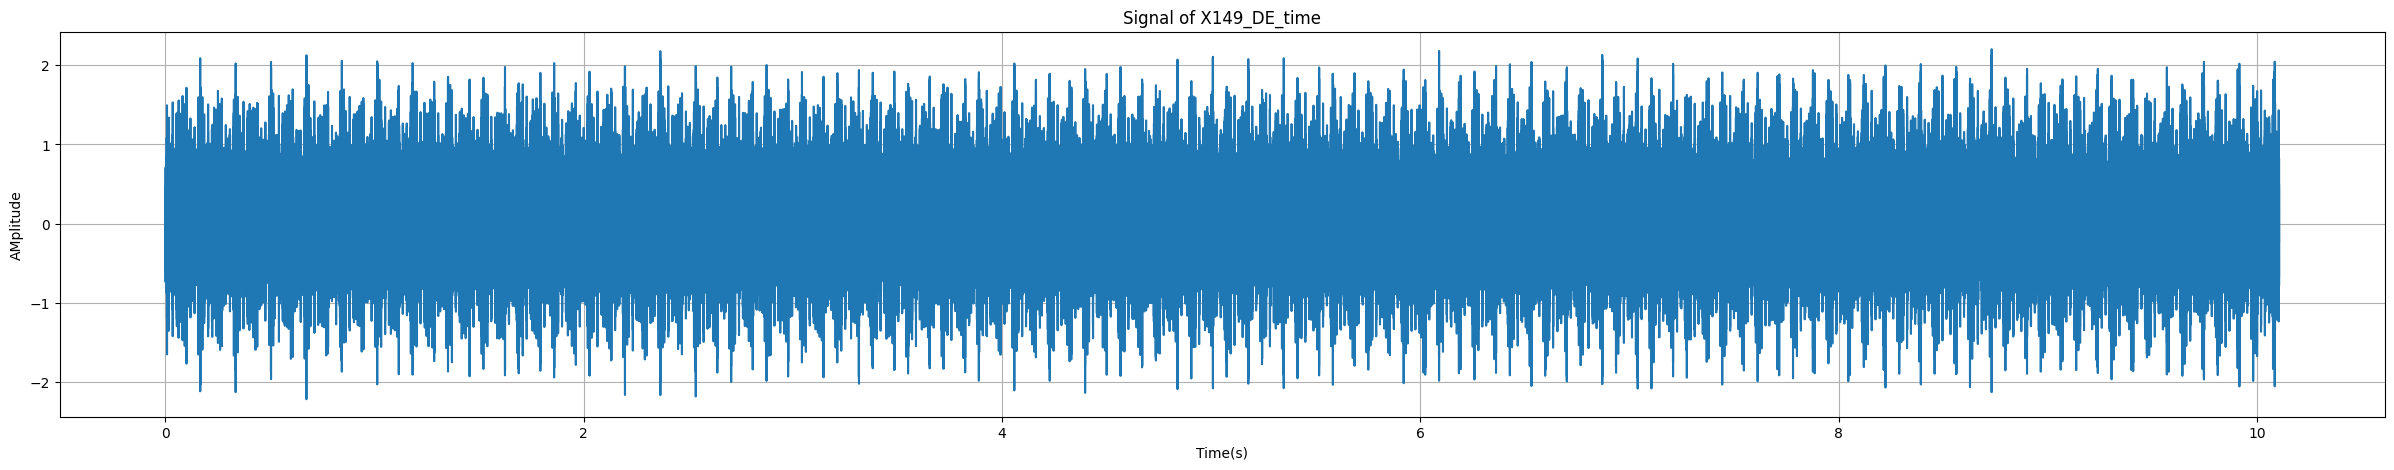
\includegraphics[width=1\linewidth]{../img/1}
	\caption{نمودار سیگنال $X149_DE_time$}
	\label{fig:1_}
\end{figure}

در بخش بعد، با محدود کردن ناحیه ی x در نمودار بین بازه ی 2 تا 2.01 ثانیه، سیگنال را مشاهده می کنیم.
\begin{minted}{python}
time = np.linspace(0, len(DE_time)/fs, len(DE_time))
plt.figure(figsize=(30, 5))
plt.plot(time, DE_time)
plt.xlabel("Time(s)")
plt.xlim(2, 2.01)
plt.ylabel("Amplitude") 
plt.title("Signal of X149_DE_time")
plt.grid(True)
plt.show()
\end{minted}
% TODO: \usepackage{graphicx} required
\begin{figure}[H]
	\centering
	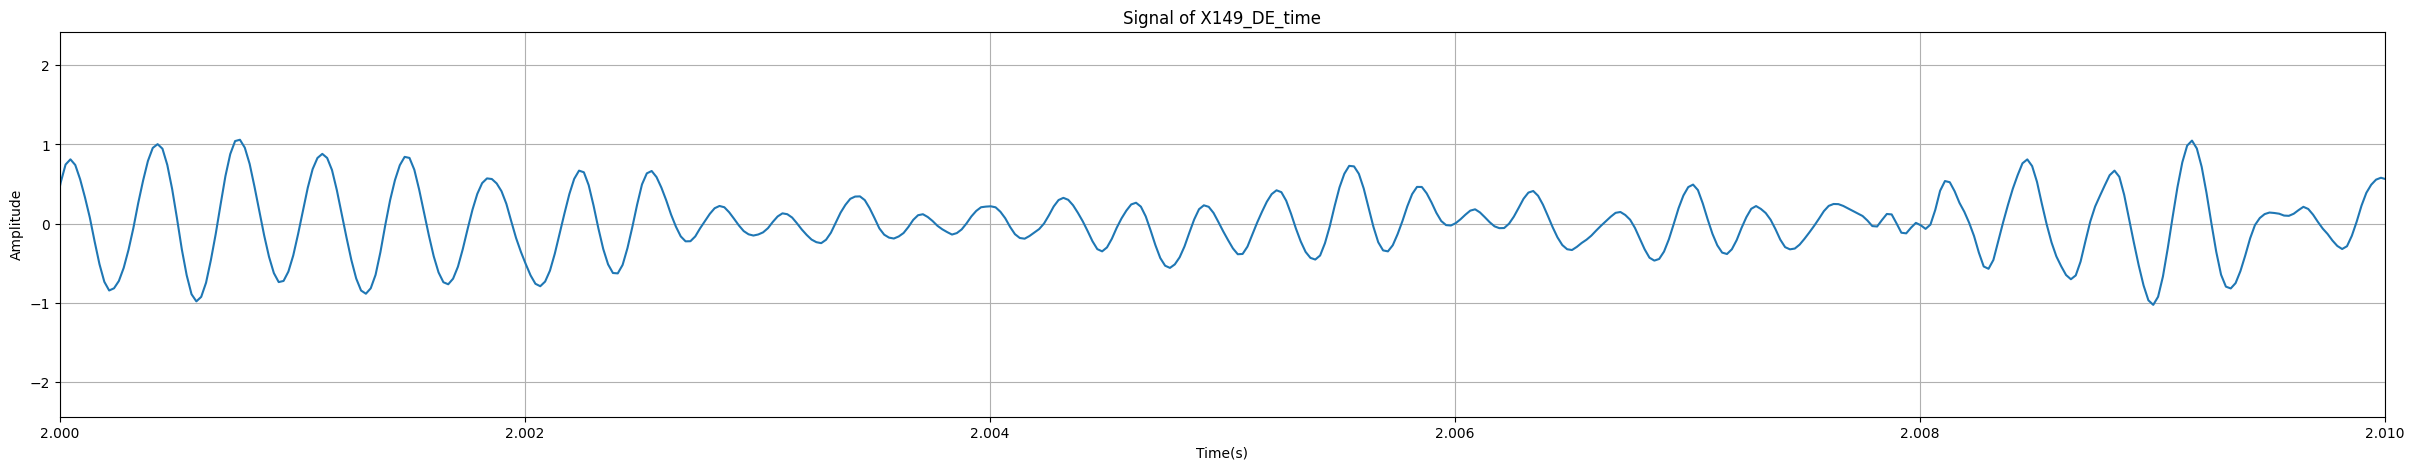
\includegraphics[width=1\linewidth]{../img/2}
	\caption{نمودار در بازه  ی2 تا $2.01$ ثانیه}
	\label{fig:2_}
\end{figure}

\subsection{بخش ج، تحلیل فرکانسی}
در این بخش، تابعی برای محاسبه ی تبدیل فوریه نوشته می شود. در نوشتن این تابع از روش fft در پکیج numpy استفاده شده است و پس از مشخص کردن فرکانس نمونه برداری داده ها، نمودار حوزه فرکانس سیستم رسم شده است.


% TODO: \usepackage{graphicx} required
\begin{figure}
	\centering
	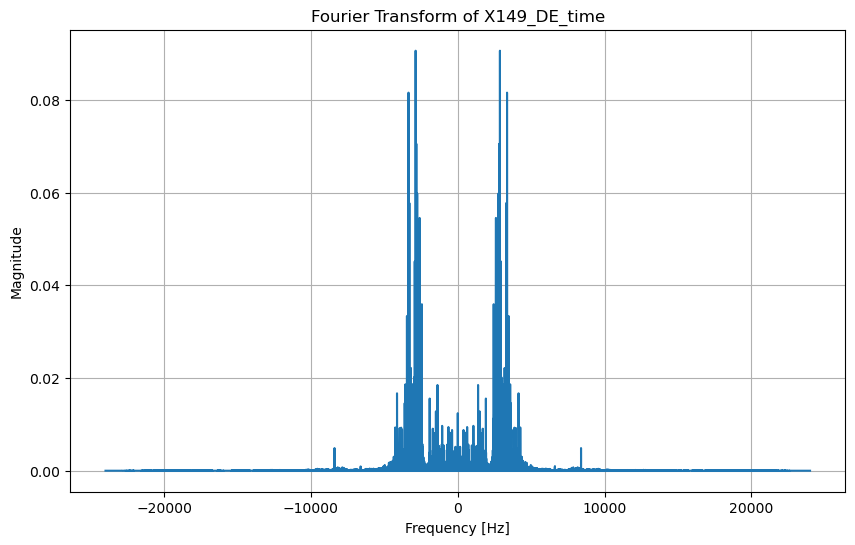
\includegraphics[width=1\linewidth]{../img/3}
	\caption{نمودار حوزه فرکانس سیگنال مورد بررسی}
	\label{fig:3_}
\end{figure}
همچنین، با اندازه گیری فرکانس با بیشترین دامنه، فرکانس غالب سیستم را برابر با
$3201 Hz$ به دست می آوریم.

\subsection{بخش د و ه، تقسیم بندی سیگنال}
برای تقسیم سیگنال به سطر هایی با 128 نمونه، از دستور reshape استفاده می کنیم. با این حال، باید توجه داشته باشیم که تعداد داده ها باید حتما بر 128 بخش پذیر باشند و بنابراین، پیش از اعمال دستور reshape، سیگنال را به تعدادی بخش پذیر بر 128 برش می دهیم. 
در نهایت، ماتریسی به صورت زیر به دست می آید.
\begin{minted}{python}
num_sections = len(DE_time) // 128
signal_trimmed = DE_time[:num_sections * 128]
sections = signal_trimmed.reshape(-1,128)
df = pd.DataFrame(sections)
df
\end{minted}
\begin{figure}
	\centering
	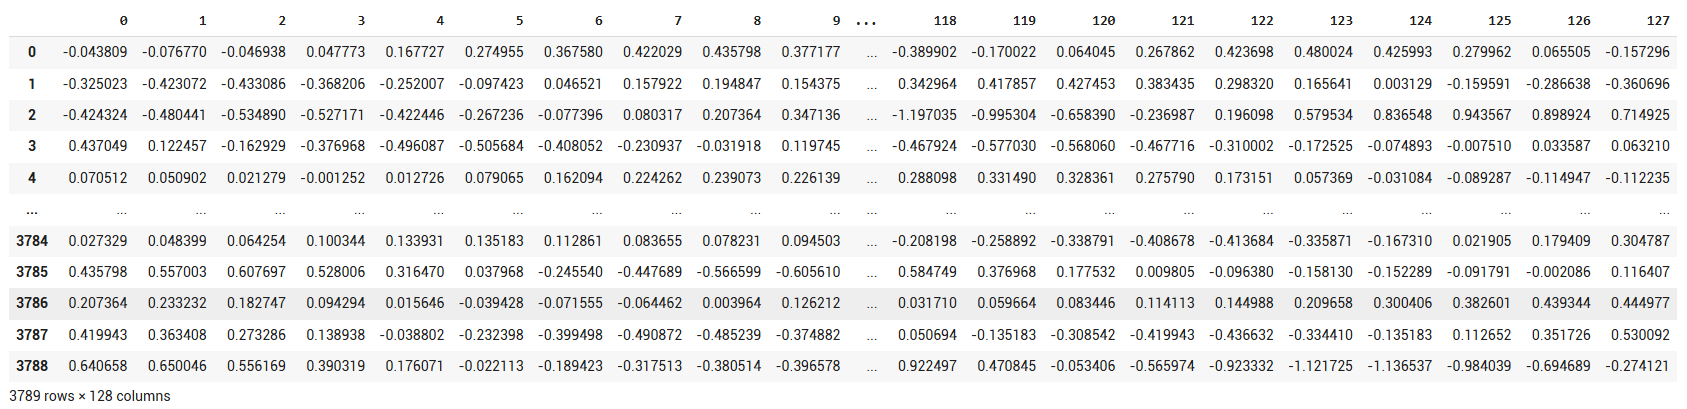
\includegraphics[width=1\linewidth]{../img/4}
	\caption{دیتافریم بخش های سیستم}
	\label{fig:4_}
\end{figure}

در نهایت، برای رسم نمودار بخش های انتخاب شده از سیگنال، با استفاده از کتابخانه ی matplotlib، آنها را در یک حلقه ی for به نمودار اضافه کرده و در نهایت نمودار را نمایش می دهیم. لازم به ذمر است که برای اضافه کردن legend به سیستم نیز، برای هر نمودار label متناسب تولید کرده و در نهایت، آن را در legend نمایش می دهیم.
\begin{minted}{python}
plt.figure(figsize=(10, 5))
for i in range(10):
var = df.iloc[13*i]
var = np.array(var).reshape(var.shape[0], -1)  
plt.plot(np.arange(len(var)), var.flatten(), label=f"Section {i+1}")  
plt.title("Sections")
plt.xlabel("Samples")
plt.ylabel("Value")
plt.legend(loc="center left", bbox_to_anchor=(1, 0.5)) 
plt.tight_layout()  
plt.show()
\end{minted}
نمودار به دست آمده آنگاه به صورت زیر خواهد بود.
\begin{figure}[H]
	\centering
	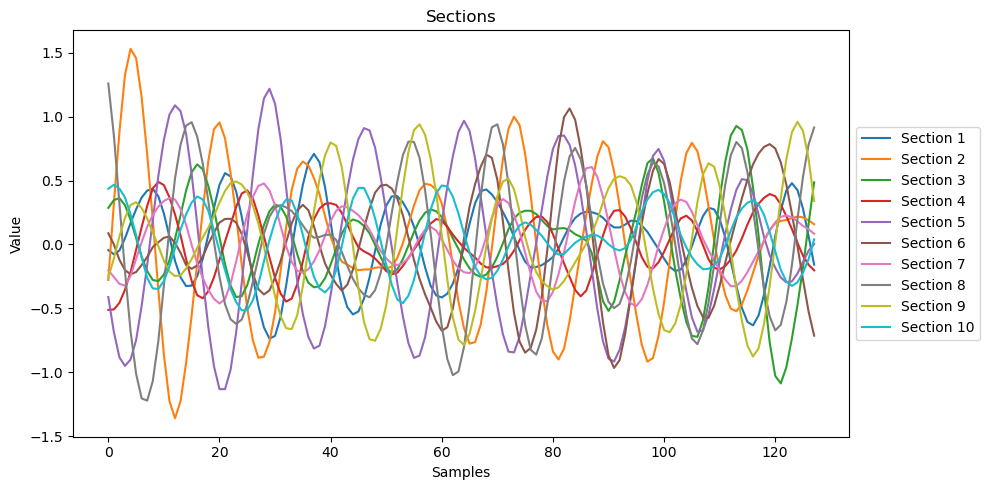
\includegraphics[width=1\linewidth]{../img/5}
	\caption{نمودار بخش های جدا شده از سیستم بر حسب زمان}
	\label{fig:5_}
\end{figure}

\subsection{بخش و، استخراج ویژگی}
در این قسمت، ویژگی های میانگین، انحراف معیار و RMS را با استفاده از روش های موجود در کتابخانه ی numpy محاسبه می کنیم. برای این کار، در یک class، تابع های مورد نیاز را تعریف کرده و سپس در پایان آن، در تابع main، هر سه را فراخوانی می کنیم. برای محاسبه ی میانگین و انحراف معیار از روش های آماده در کتابخانه ی numpy استفاده شده و RMS به صورت مجزا تعریف شده است.

\begin{minted}{python}
class Statistics:
def __init__(self, signal):
self.signal = np.array(signal)

def mymean(self):
return np.mean(self.signal)

def mystddev(self):
return np.std(self.signal)

def myRMS(self):
return np.sqrt(np.mean(np.square(self.signal)))

def main(signal):
stats = Statistics(signal)
print("Mean:", stats.mymean())
print("Standard Deviation:", stats.mystddev())
print("RMS:", stats.myRMS())
\end{minted}
	
آنگاه با فراخوانی این تابع و اعمال ورودی سیگنال به آن، می توانیم جدول ویژکی ها را محاسبه کنیم.

برای ایجاد ویژگی های خواسته شده برای تمام نمونه ها در دیتافریم، با فرض اینکه آن ستون ها وجود دارند، مقادیر را مطابق با روش های موجود در کلاس ساخته شده و به وسیله ی $lamda function$ می نویسیم.
\begin{minted}{python}
	df['Mean'] = df.apply(lambda row: Statistics(row.values).mymean(), axis = 1)
\end{minted}
	
\begin{minted}{python}
df['Standard Deviation'] = df.apply(lambda row: Statistics(row.values).mystddev(), axis = 1)
df['RMS'] = df.apply(lambda row: Statistics(row.values).myRMS(), axis = 1)
df
df.tocsv("dataset.csv", index=False)
\end{minted}
در پایان، دیتافریم به صورت زیر قابل مشاهده خواهد بود.
\begin{figure}[H]
	\centering
	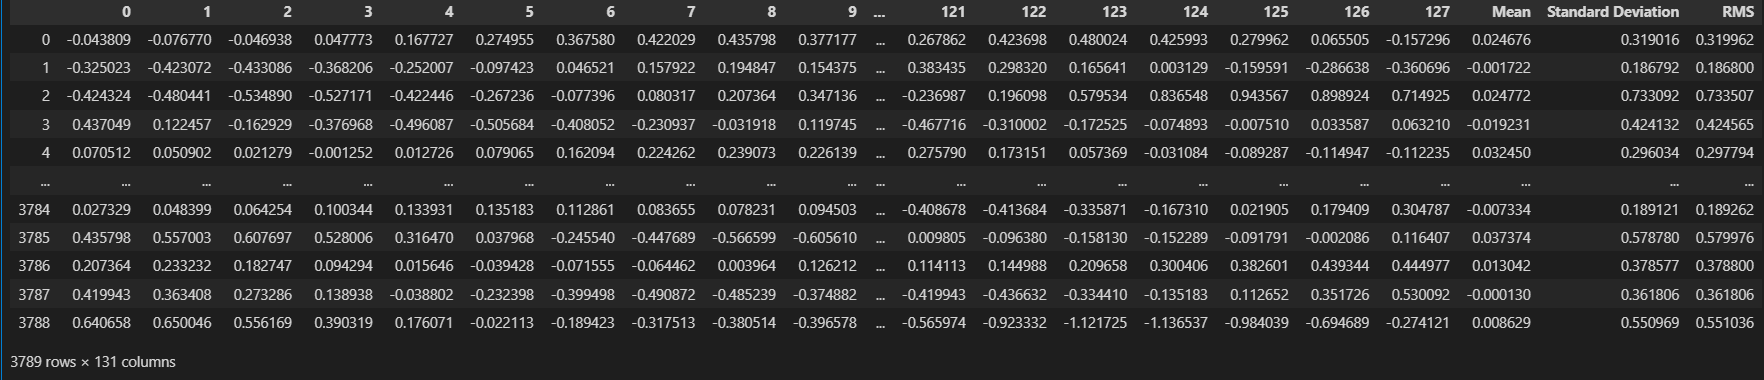
\includegraphics[width=1\linewidth]{../img/6}
	\caption{دیتافریم پس از استخراج ویژگی}
	\label{fig:6}
\end{figure}
در نهایت، دیتافریم را در یک فایل csv ذخیره می کنیم.
\section{پاسخ سوال سوم، قسمت دوم}
\subsection{بخش اول، بررسی اولیه}
دیتاست گل زنبق اولین بار توسط رونالد فیشر در کتابش معرفی شد و شامل داده های 150 نمونه گل زنبق است. ویژگی های اندازه گیری شده برای این گل ها به شرح زیر است:
\begin{enumerate}
	\item Sepal Length
	\item Sepal Width
	\item Petal Length
	\item Petal Width
\end{enumerate}
که مربوط به ابعاد اجزای گل ها می باشد. علاوه بر این، سه کلاس مختلف این گل ها به صورت زیر در این دیتاست نام گذاری شده اند:
\begin{enumerate}
	\item 0: Setosa
	\item 1: Versicolor
	\item 2: Virginica
\end{enumerate}

از ویژگی های بارز این دیتاست آن است که به ازای هر کلاس، دقیقا 50 نمونه داده وجود دارد که دیتاست را متعادل می سازد. علاوه بر این، داده ی خالی ندارد و همچنین کلاس Setosa به صورت خطی قابل جداسازی است.
برای استفاده از این دیتاست، می توانیم آن را از کتابخانه ی scikit-learn فراخوانی کنیم. در این دستور، از مجموعه داده های موجود در کتابخانه ی $scikit-learn$ دیتاست Iris را فراخوانده و سپس آن را در یک دیتافریم ذخیره می کنیم.
\begin{minted}{python}
	from sklearn import datasets
	import pandas as pd
	
	# Load dataset
	iris = datasets.load_iris()
	df = pd.DataFrame(iris.data, columns=iris.feature_names)
	df['species'] = iris.target
	
	print(df.head())
\end{minted}
% TODO: \usepackage{graphicx} required
\begin{figure}[H]
	\centering
	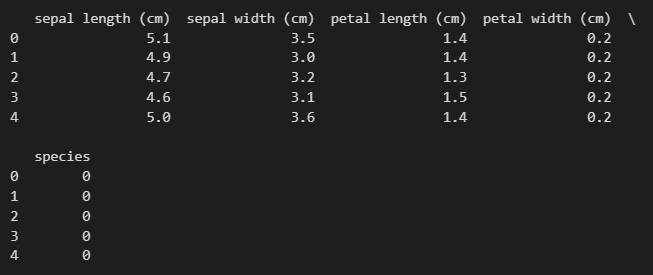
\includegraphics[width=0.7\linewidth]{../img/7}
	\caption{نمونه داده ی دیتاست زنبق}
	\label{fig:7}
\end{figure}

در ادامه برای تقسیم دیتاست به بخش آموزشی و تست، با استفاده از روش $Train_Test_split$ از کتابخانه ی sklearn در بخش $model_selection$ داده ها را به دو بخش تقسیم می کنیم. در اینجا ابتدا مقادیر فیچرها و کلاس های خروجی را به عنوان ورودی و خروجی سیستم تعریف کرده و سپس با استفاده از دستور ذکر شده، آنها را تقسیم می کنیم.
\begin{minted}{python}
	from sklearn.model_selection import train_test_split
	
	X = iris.data
	y = iris.target
	
	X_train, X_test, y_train, y_test =
	train_test_split(X,y, test_size=0.15, random_state=43) 
\end{minted}
در ادامه، نام ستون های متغیر های به دست آمده را باید مجدد نام گذاری کنیم و البته آنها را در دیتافریم هایی ذخیره کنیم.
\begin{minted}{python}
X_train = pd.DataFrame(X_train)
X_train.rename(columns={0:'Sepal Length',
 1:"Sepal Width",
 2:"Petal Length",
 3:"Petal Width"},inplace=True)

X_test = pd.DataFrame(X_test)
X_test.rename(columns={0:'Sepal Length',
 1:"Sepal Width",
 2:"Petal Length",
 3:"Petal Width"},inplace=True)

y_train = pd.DataFrame(y_train)
y_train.rename(columns={0:'Iris Type'},inplace=True)

y_test = pd.DataFrame(y_test)
y_test.rename(columns={0:'Iris Type'},inplace=True)

\end{minted}

در نهایت، دیتافریم های آموزش و تست را با به هم پیوستن داده های x و y آنها به وسیله دستور concat ترکیب می کنیم. 
\begin{minted}{python}
Train_df = pd.concat([X_train,y_train], axis=1)
Test_df = pd.concat([X_test,y_test], axis=1)
\end{minted}
برای مشخص کردن آنکه داده ها، مربوط به تست و یا آموزش هستند، ستونی به هر یک از دیتافریم ها با عنوان $is train$ اضافه شده که برای داده های train دارای مقدار 1 و برای داده های تست دارای مقدار 0 است.
در نهایت، با استفاده ی مجدد از دستور concat و به هم پیوستن این دو دیتافریم، دیتاست به صورت زیر به دست می آید.
\begin{minted}{python}
temporary_train = Train_df
temporary_train["is train"] = 1
temporary_test = Test_df
temporary_test["is train"] = 0

Dataset = pd.concat([temporary_train,temporary_test],ignore_index=True)
\end{minted}
\begin{figure}[H]
	\centering
	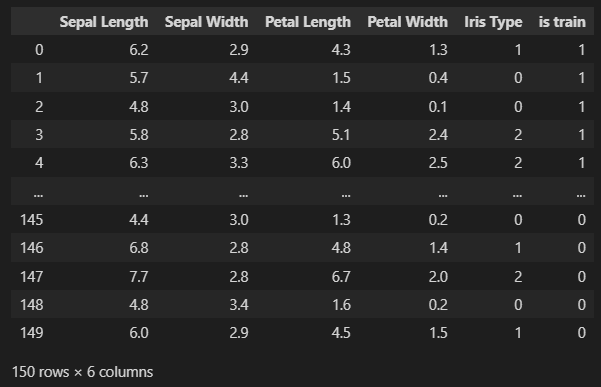
\includegraphics[width=0.7\linewidth]{../img/8}
	\caption{دیتاست}
	\label{fig:8}
\end{figure}
\subsection{تحلیل بصری داده}
در این بخش با در اختیار داشتن دیتاست، به رسم نمودار هایی از دیتاست و مشاهده داده های موجود در آن می پردازیم.
در بخش اول، دو ویژگی $Petal Length$ و $Petal Width$ از دیتاست را انتخاب کرده و توزیع آنها را نمایش می دهیم. این کار با استفاده از دستور jointplot از کتابخانه ی seaborn انجام می شود.
\begin{minted}{python}
import seaborn as sns
sns.jointplot(x=Dataset["Petal Length"], y=Dataset["Petal Width"],

kind="scatter", hue=Dataset["Iris Type"],palette="coolwarm")
\end{minted}
% TODO: \usepackage{graphicx} required
\begin{figure}[H]
	\centering
	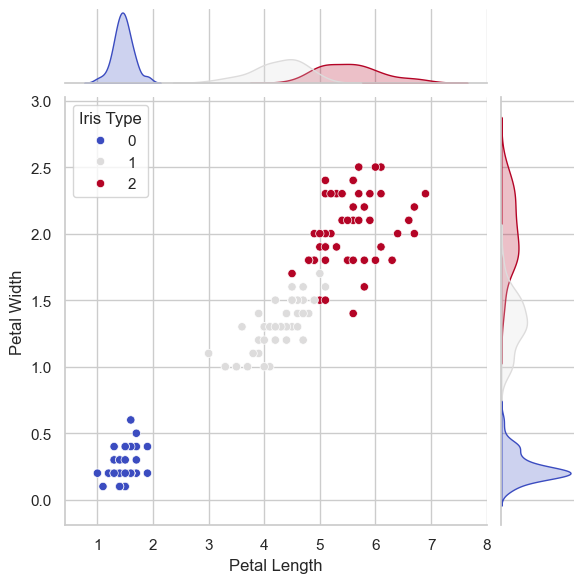
\includegraphics[width=1\linewidth]{../img/9}
	\caption{توزیع داده های $Petal Length$ و $Petal Width$ }
	\label{fig:9}
\end{figure}
در ادامه برای نمایش سه ویژگی از این دیتاست در یک نمودار سه بعدی به تفکیک نوع زنبق ها، از کتابخانه ی plotly استفاده می کنیم. در این روش، مقادیر دیتافریم در سه متغیر x و y و z تعریف شده و رنگ آن بر اساس نوع زنبق تعیین می شود.
پس از تعیین نمودار و برای بهبود آن، مارکر های قرار داده شده را تنظیم می کنیم و رنگ حاشیه آنها و ضخامت را تعیین می کنیم.
\begin{minted}{python}
import plotly.express as px

# Create the 3D scatter plot
fig = px.scatter_3d(Dataset,
x="Petal Length",
y="Petal Width",
z="Sepal Width",
color="Iris Type",  # Different colors for each species
color_discrete_sequence=px.colors.sequential.Magma, 
title="3D Scatter Plot of Iris Dataset")

# Customize markers
fig.update_traces(marker=dict(size=5,  # Marker size
opacity=0.8,  # Transparency
line=dict(width=10, color='black')),  # Black border around each point
selector=dict(mode='markers'))

# Add interactive layout settings
fig.update_layout(margin=dict(l=0, r=0, b=0, t=40),  # Remove margins
scene=dict(aspectmode='cube'))  # Equal scaling on all axes

# Show plot
fig.show()
\end{minted}
% TODO: \usepackage{graphicx} required
\begin{figure}[H]
	\centering
	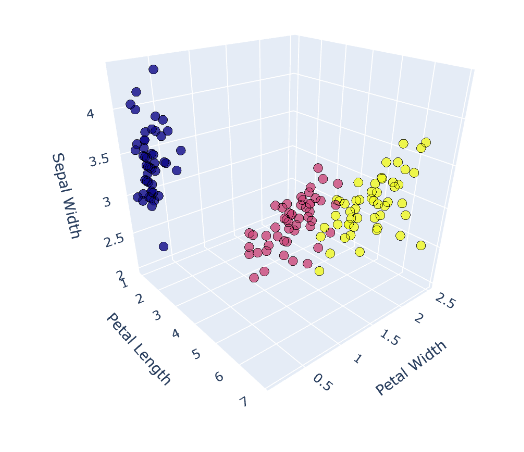
\includegraphics[width=0.7\linewidth]{../img/10}
	\caption{توزیع داده های سه وِیژگی سیستم}
	\label{fig:10}
\end{figure}
% TODO: \usepackage{graphicx} required
\begin{figure}[H]
	\centering
	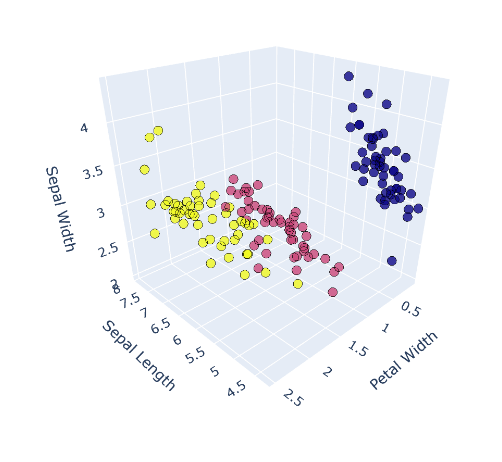
\includegraphics[width=0.7\linewidth]{../img/11}
	\caption{توزیع داده ها با سه ویژگی دیگر}
	\label{fig:11}
\end{figure}

در بخش بعد، برای بررسی شباهت فیچر های دیتاست با یکدیگر، ابتدا مقدار correlation آنها را به دست آورده و سپس نقشه حرارتی آن را رسم می کنیم.
\begin{minted}{python}
sns.heatmap(Dataset.corr(),annot=True )
plt.title("Correlation Heatmap")
\end{minted}
% TODO: \usepackage{graphicx} required
\begin{figure}[H]
	\centering
	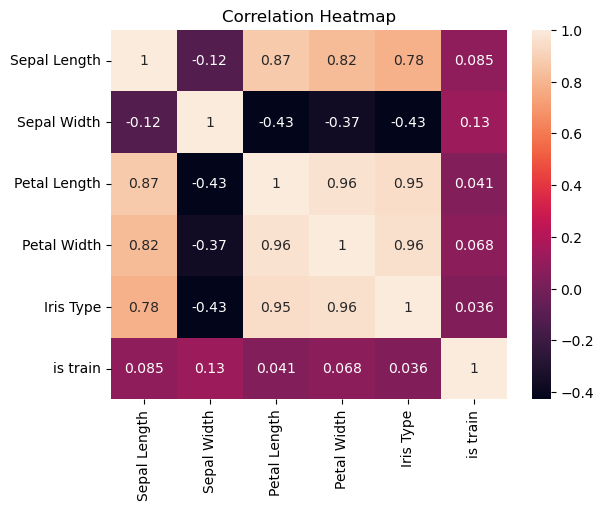
\includegraphics[width=0.7\linewidth]{../img/12}
	\caption{نمودار حرارتی correlation}
	\label{fig:12}
\end{figure}
در بخش بعد، به نمایش توزیع داده های هر فیچر به تفکیک داده های آموزش و تست می پردازیم. برای به دست آوردن این نمودارها، از دستور pairplot استفاده می شود. با اجرای این دستور برای دیتاست، توزیع دو به دوی تمامی فیچر ها نمایش داده می شود که بر روی قطر اصلی، توزیع هر ویژگی قابل مشاهده است.
\begin{minted}{python}
sns.pairplot(Dataset,hue='is train',palette='coolwarm')
\end{minted}
% TODO: \usepackage{graphicx} required
\begin{figure}[H]
	\centering
	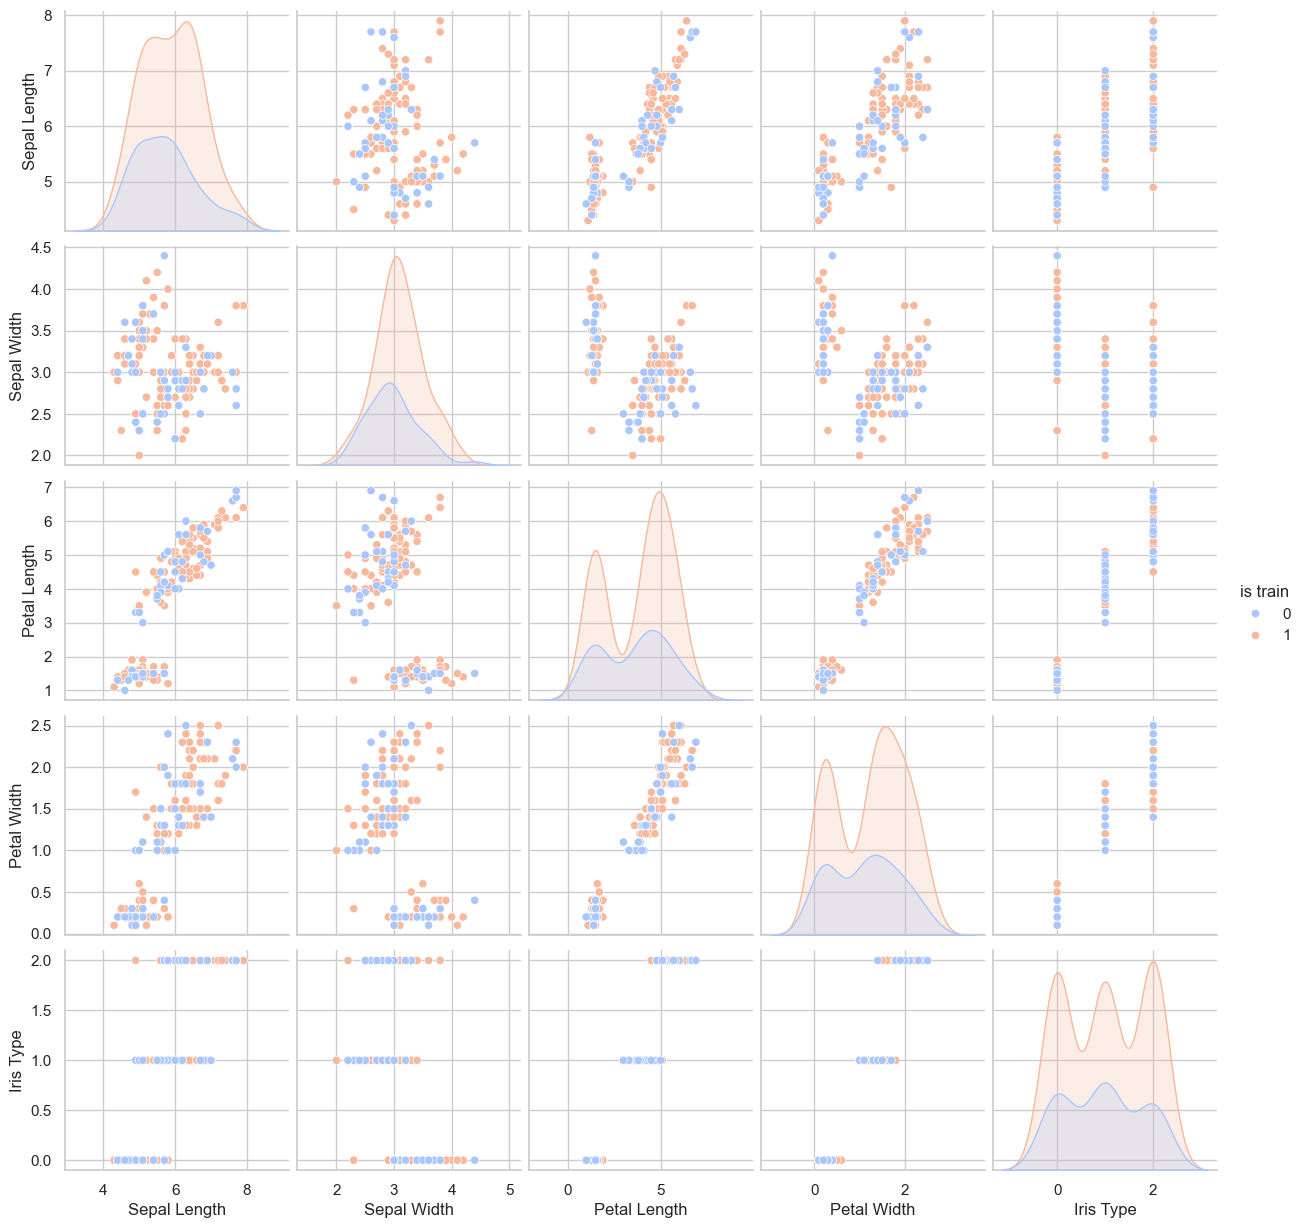
\includegraphics[width=1\linewidth]{../img/13}
	\caption{$Pair Plot$}
	\label{fig:13}
\end{figure}
\subsection{گسسته سازی}
در این بخش، ویژگی $petal length$ را گسسته می کنیم. برای این کار، تعداد دسته های مورد نیاز و عنوان آنها را تعریف کرده و سپس با استفاده از دستور cut از کتابخانه ی pandas، مقادی را در بازه های مورد نظر دسته بندی می کنیم.
\begin{minted}{python}
bins = 3  # Number of categories
labels = ["Short", "Medium", "Tall"]  # Custom labels
Dataset["Discrit Petal Lemgth"]=pd.cut(Dataset["Petal Length"], bins=bins, labels=labels)
\end{minted}
در این صورت، دیتاست نهایی به صورت زیر به دست می آید.
% TODO: \usepackage{graphicx} required
\begin{figure}[H]
	\centering
	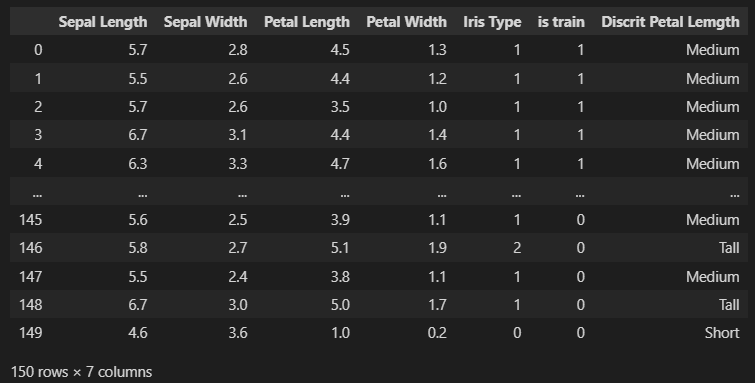
\includegraphics[width=0.7\linewidth]{../img/14}
	\caption{دیتاست پس از گسسته سازی}
	\label{fig:14}
\end{figure}
\subsection{تحلیل آماری}
در گام آخر، دیتاست را با استفاده از متد describe، توصیف کرده و پارامتر های آماری آن را محاسبه می کنیم. در اینجا تنها شرط آن را قرار می دهیم که تنها داده هایی با $Iris Type$ برابر با 0 که معادل Setosa است آورده شود.
\begin{minted}{python}
Dataset[Dataset["Iris Type"] ==0].describe()
\end{minted}
% TODO: \usepackage{graphicx} required
\begin{figure}[H]
	\centering
	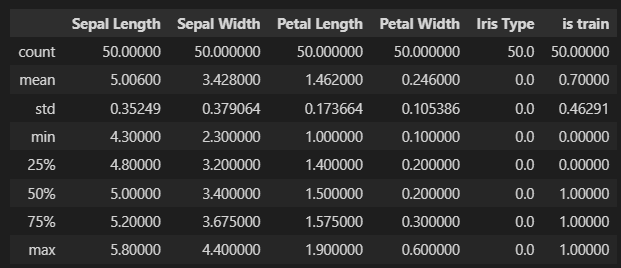
\includegraphics[width=0.7\linewidth]{../img/15}
	\caption{تحلیل آماری داده های ستوسا}
	\label{fig:15}
\end{figure}







	



 
 
 
 		% فصل اول: مقدمه
%\include{./tex/chapter2}		% فصول دوم: مروری بر مطالعات انجام شده
%\include{./tex/chapter3}		% فصل سوم: معرفی معماری POLO
%% !TeX root=../main.tex

\chapter*{پاسخ سوالات سری چهارم}

% دستور زیر باعث عدم‌نمایش شماره صفحه در اولین صفحهٔ این فصل می‌شود.
%\thispagestyle{empty}
\section*{ پاسخ سوال 1}
\subsection*{بخش یکم}

در سوال اول با توجه به معادلات حالت سیستم که به صورت زیر داده شده است، می توانیم درکی از سیستم به دست بیاوریم:]
\[
\begin{bmatrix}
	\dot{x}_1 \\ \dot{x}_2 \\ \dot{x}_3 \\ \dot{x}_4
\end{bmatrix}
=
\begin{bmatrix}
	0 & 1 & 0 & 0 \\
	0 & -\frac{c_S}{M_S} & \frac{k_S}{M_S} & \frac{c_S}{M_S} \\
	0 & 0 & 1 & 0 \\
	-\frac{k_U}{M_U} & \frac{c_S}{M_U} & \frac{k_S + k_U}{M_U} & \frac{-c_S + c_U}{M_U}
\end{bmatrix}
\begin{bmatrix}
	x_1 \\ x_2 \\ x_3 \\ x_4
\end{bmatrix}
+
\begin{bmatrix}
	0 \\ \frac{c_S c_U}{M_S M_U} \\ -\frac{c_U}{M_U} \\ \frac{c_U}{M_U}\left(\frac{k_U}{c_U} - \frac{c_S}{M_U} - \frac{c_U}{M_U}\right)
\end{bmatrix}
d
+
\begin{bmatrix}
	0 \\ \frac{1}{M_S} \\ 0 \\ -\frac{1}{M_U}
\end{bmatrix}
u
\]

\[
\begin{bmatrix}
	y_1 \\ y_2 \\ y_3
\end{bmatrix}
=
\begin{bmatrix}
	1 & 0 & 0 & 0 \\
	0 & 1 & 0 & 0 \\
	0 & 0 & 1 & 0
\end{bmatrix}
\begin{bmatrix}
	x_1 \\ x_2 \\ x_3 \\ x_4
\end{bmatrix}
+
\begin{bmatrix}
	0 \\ 0 \\ 0
\end{bmatrix}
d
+
\begin{bmatrix}
	0 \\ 0 \\ 0
\end{bmatrix}
u
\]

مشاهده می شود که سیستم دارای چهار حالت و سه خروجی مشاهده پذیر است.
ساختار کنترلی پیش بین خطی برای این سوال به صورت زیر طراحی می شود.
\begin{figure}[H]
	\centering
	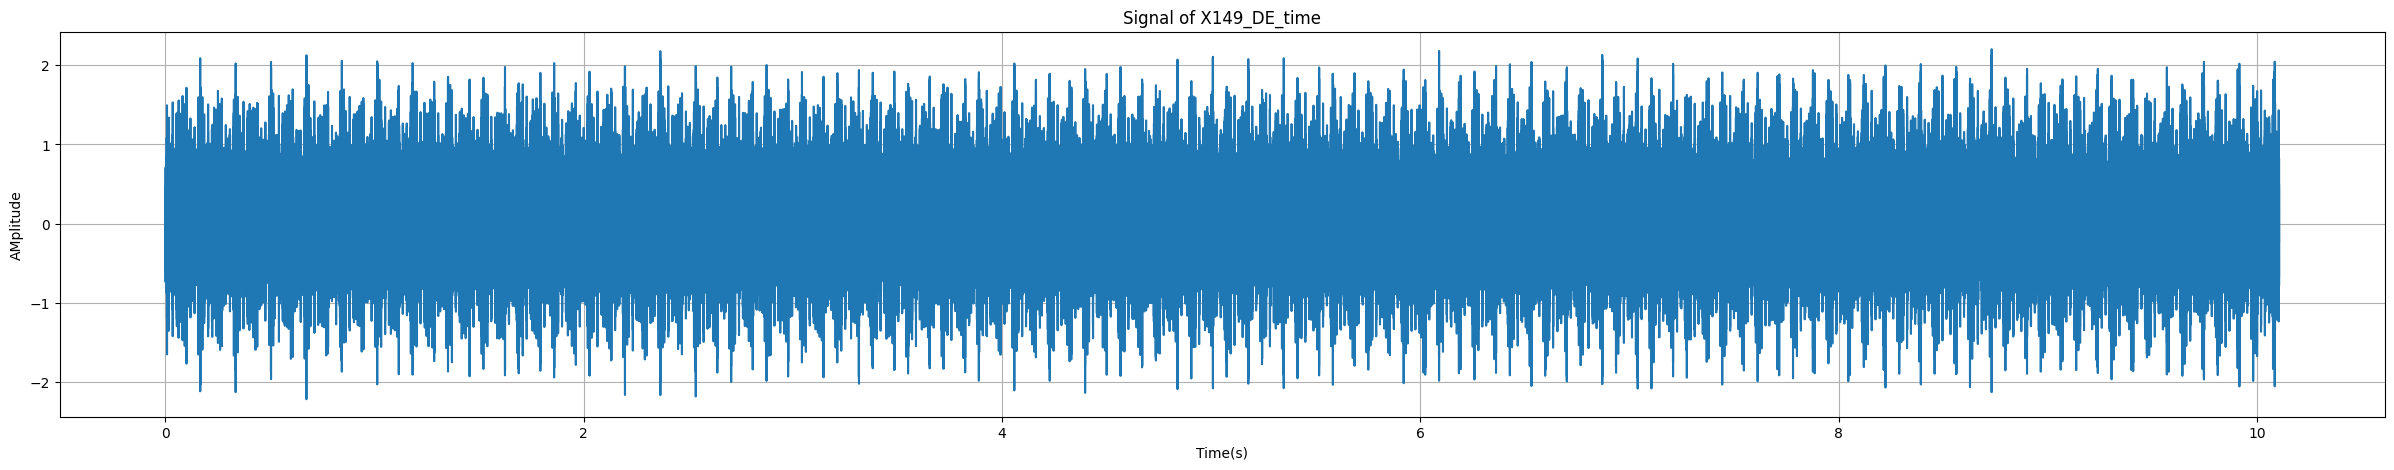
\includegraphics[width=1\linewidth]{../img/1}
	\caption{بلوک دیاگرام LMPC}
	\label{fig:1}
\end{figure}
لازم به ذکر است که با توجه به محدودیت های متلب برای ابعاد ورودی ها، خروجی ها و حالت های سیستم، چهار خروجی برای سیستم تعریف شده است، اما خروجی چهارم که نیازی نیست در نظر گرفته شود با مقدار 0 در نظر گرفته می شود.
معادلات سیستم را به صورت زیر در یک سیستم تعریف می کنیم.
\begin{figure}[H]
	\centering
	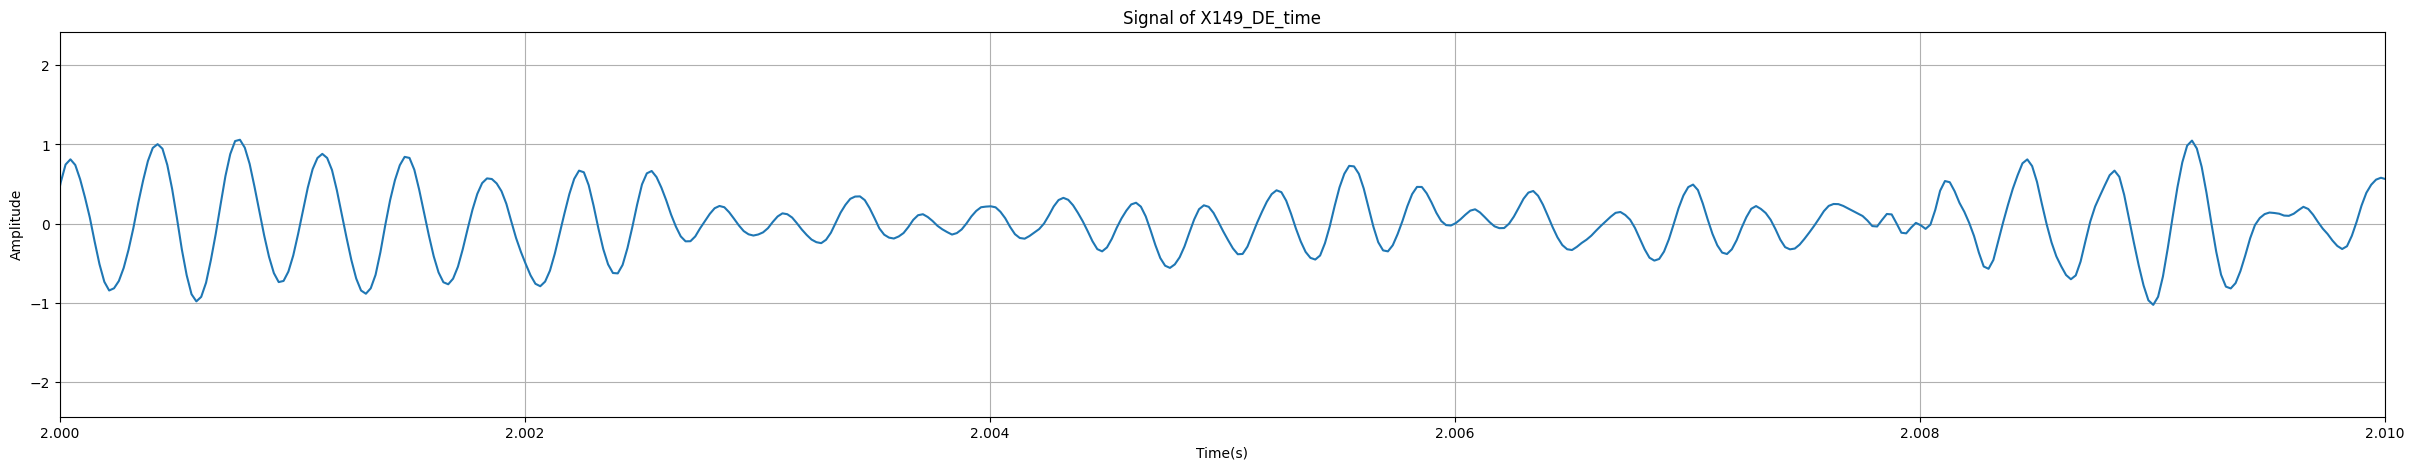
\includegraphics[width=1\linewidth]{../img/2}
	\caption{کد پلنت سیستم}
	\label{fig:2}
\end{figure}
همچنین، اغتشاش وارد شده به سیستم توسط کد زیر ایجاد می شود.

\begin{figure}[H]
	\centering
	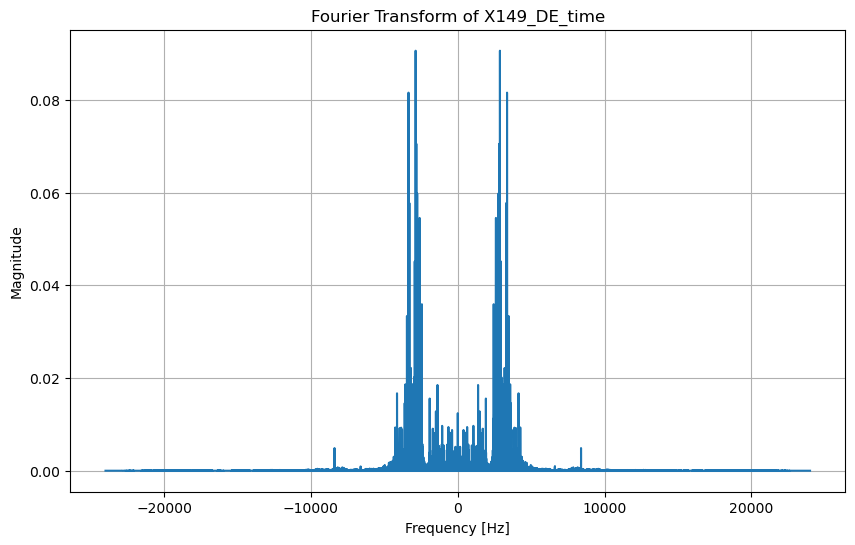
\includegraphics[width=0.4\linewidth]{../img/3}
	\caption{اغتشاش}
	\label{fig:3}
\end{figure}
در ادمه، با طراحی کنترلر MPC برای این سیستم با تنظیمات زیر، می توانیم نتایج به دست آمده از سیستم را مشاهده کنیم:

\begin{figure}[H]
	\centering
	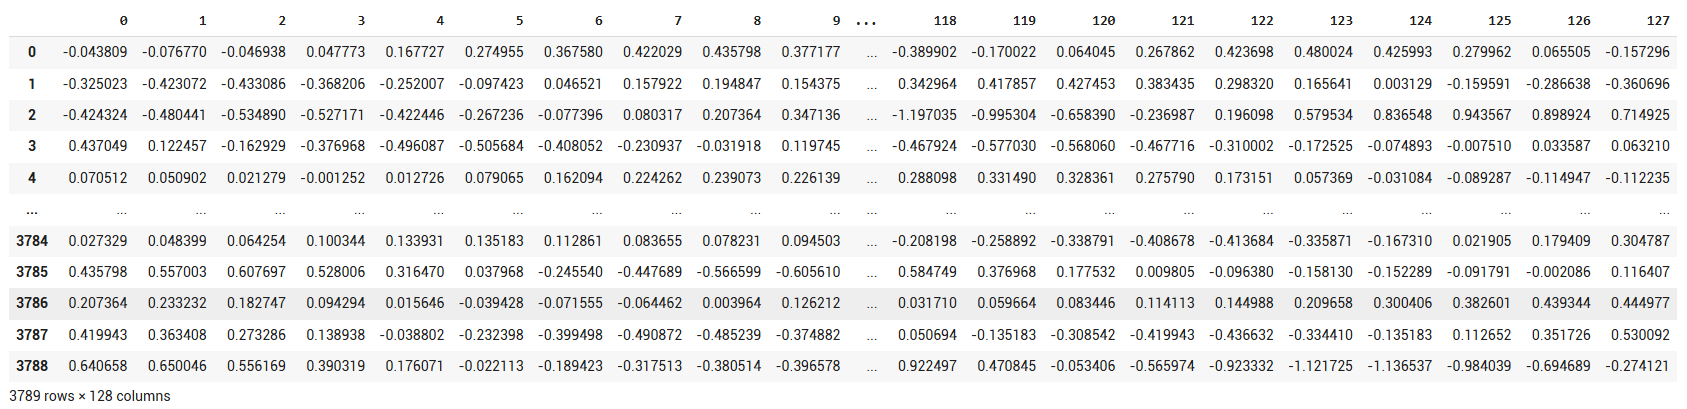
\includegraphics[width=1\linewidth]{../img/4}
	\caption{LMPC design}
	\label{fig:4}
\end{figure}
همچنین باید توجه شود که قید هایی برای حالت اول سیستم در نظر گرفته شده است تا مقدار آن از 1 بیشتر نشود. 

\begin{figure}[H]
	\centering
	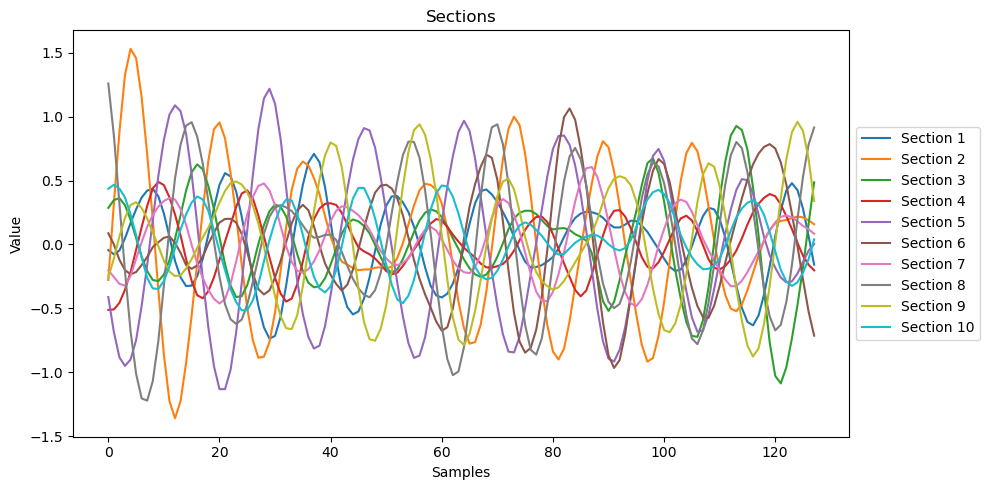
\includegraphics[width=1\linewidth]{../img/5}
	\caption{LMPC constraints configuration}
	\label{fig:5}
\end{figure}
با استفاده از سیستم تعریف شده، پاسخ های سیستم به صورت زیر به دست می آید.

\begin{figure}[H]
	\centering
	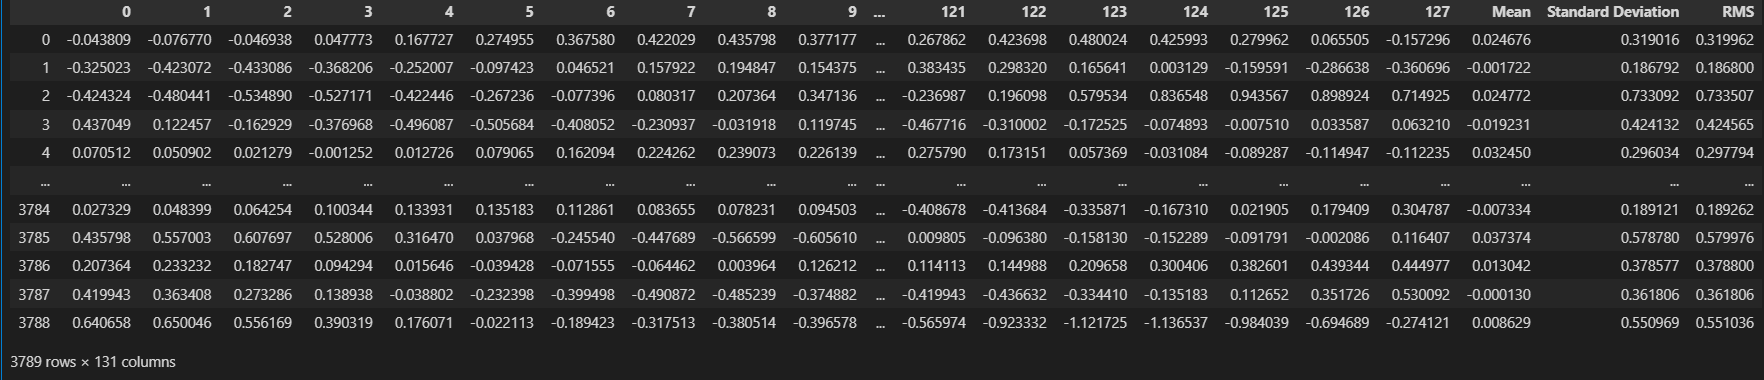
\includegraphics[width=1\linewidth]{../img/6}
	\caption{LMPC states output}
	\label{fig:6}
\end{figure}
همچنین نمودار تلاش کنترلی سیستم یه صورت زیر به دست می آید.

\begin{figure}[H]
	\centering
	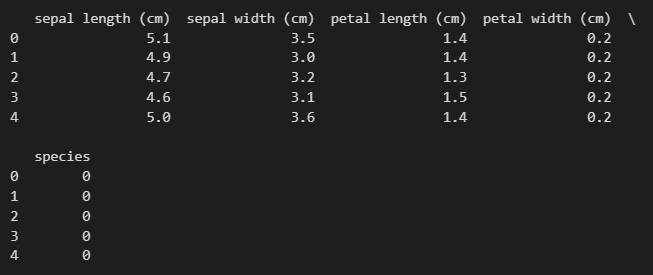
\includegraphics[width=1\linewidth]{../img/7}
	\caption{LMPC control effort}
	\label{fig:7}
\end{figure}

با در اختیار داشتن نتایج به دست آمده و به منظور تحلیل این نتایج، کنترلر PID نیز برای سیستم طراحی و بررسی می شود. دیاگرام این سیستم به شرح زیر خواهد بود:

\begin{figure}[H]
	\centering
	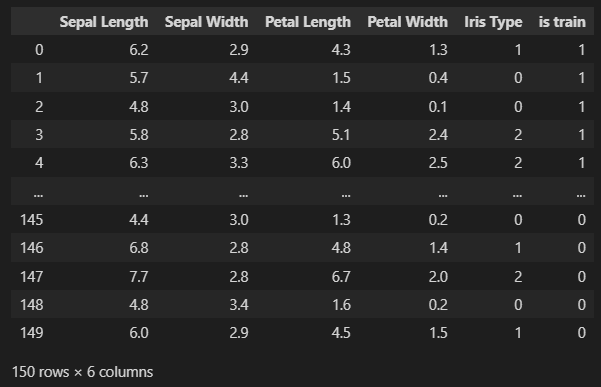
\includegraphics[width=1\linewidth]{../img/8}
	\caption{PID diagram}
	\label{fig:8}
\end{figure}

لازم به ذکر است که برای این سیستم، تنها حالت اول به عنوان خروجی سیستم در نظر گرفته شده است. پاسخ سیستم به صورت زیر به دست می آید و مشاهده می شود که می تواند به خوبی اغتشاش وارد شده را رفع کند. اما با در نظر گرفتن ضرایب PID و همچنین نمودار تلاش کنترلی مشاهده می شود که در نهایت این کنترلر در سیستم های واقعی قابل پیاده سازی نمی باشد.

\begin{figure}[H]
	\centering
	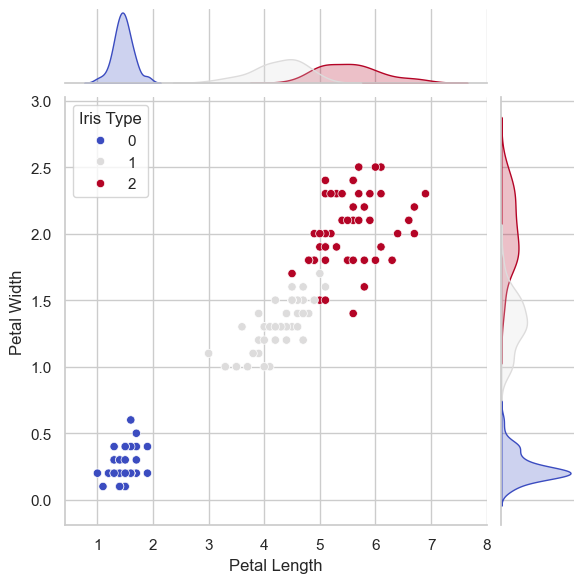
\includegraphics[width=1\linewidth]{../img/9}
	\caption{PID control effort}
	\label{fig:9}
\end{figure}

\begin{figure}[H]
	\centering
	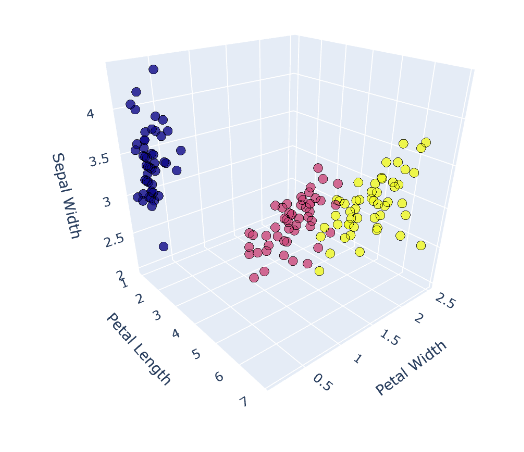
\includegraphics[width=0.7\linewidth]{../img/10}
	\caption{}
	\label{fig:10}
\end{figure}

\begin{figure}[H]
	\centering
	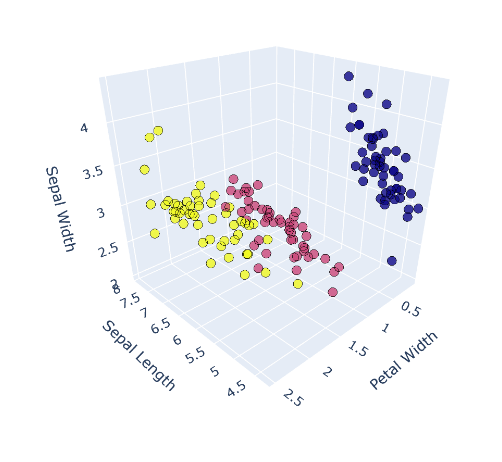
\includegraphics[width=1\linewidth]{../img/11}
	\caption{PID state1 output}
	\label{fig:11}
\end{figure}

در اینجا با در نظر گرفتن نتایج به دست آمده از MPC و PID می توانیم مقایسه ای در عملکرد آنها داشته باشیم.
نتایج به دست امده از خروجی کنترلی حالت اول با این دو کنترلر و تلاش کنترلی برای رفع آن به صورت زیر خواهد بود.

\begin{figure}[H]
	\centering
	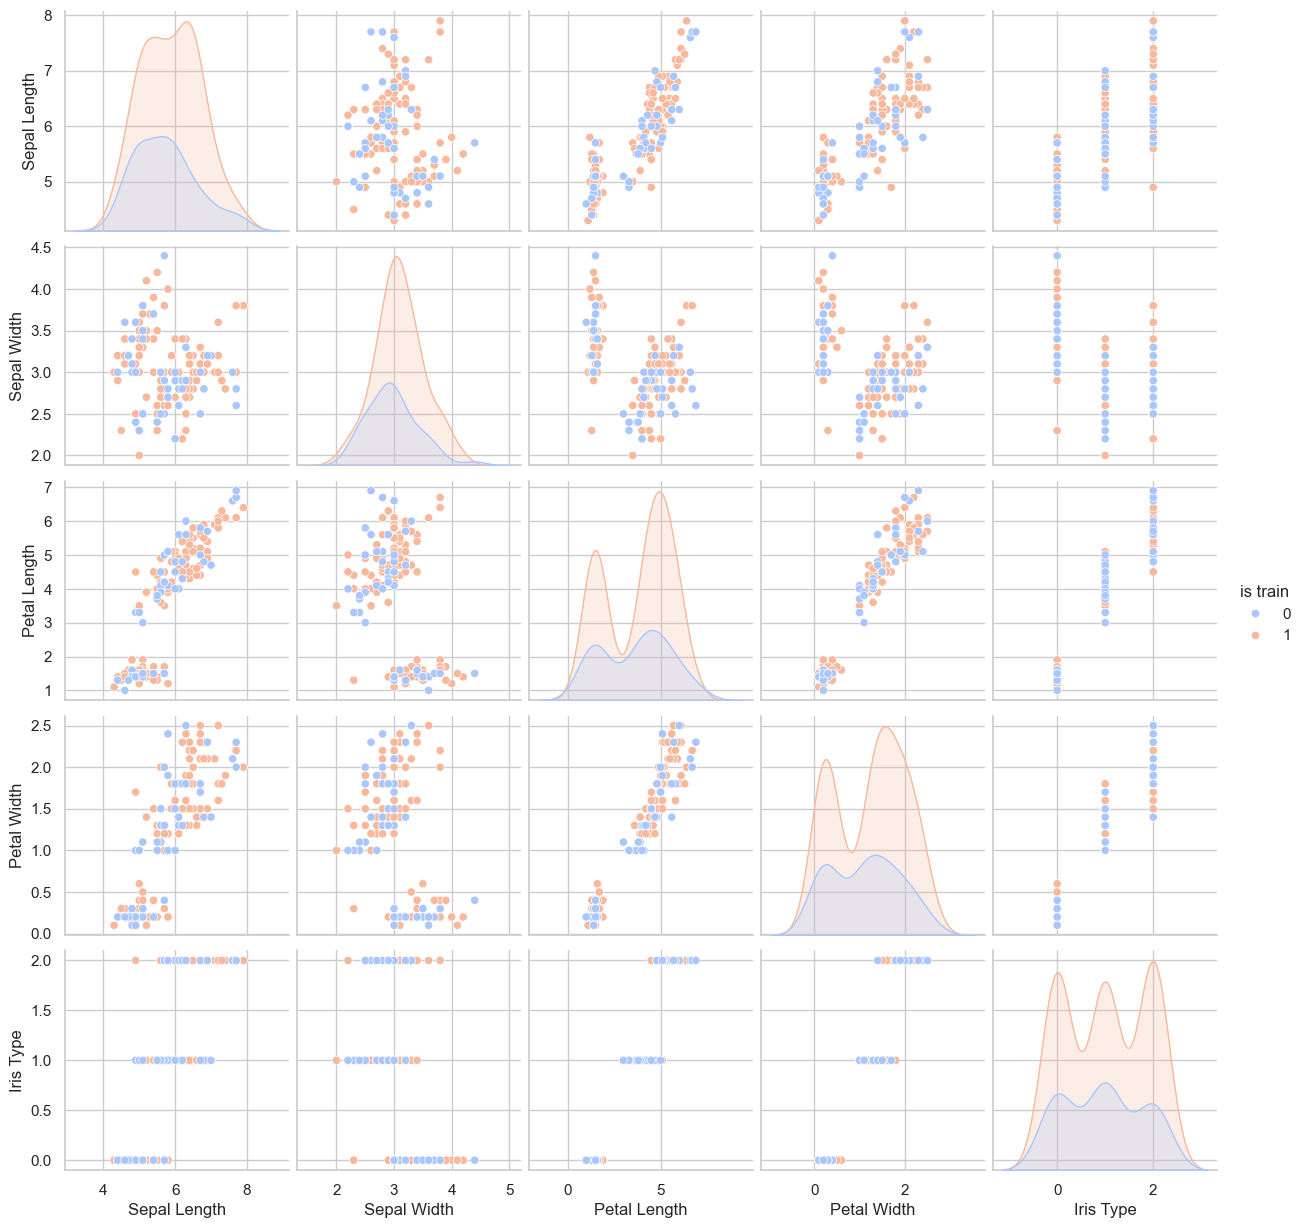
\includegraphics[width=1\linewidth]{../img/13}
	\caption{LMPC state1 output}
	\label{fig:13}
\end{figure}

\begin{figure}[H]
	\centering
	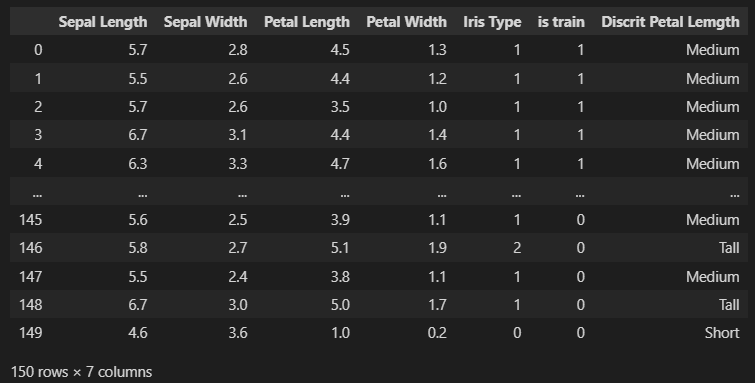
\includegraphics[width=1\linewidth]{../img/14}
	\caption{PID vs LMPC control effort}
	\label{fig:14}
\end{figure}

همچنین مقادیر RMSE برای این دو کنترلر در دو حالت مورد نظر به صورت زیر به دست می آید.

\begin{figure}[H]
	\centering
	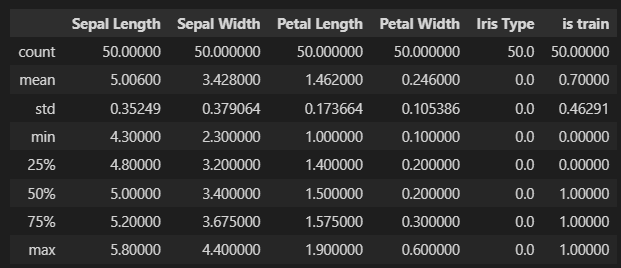
\includegraphics[width=1\linewidth]{../img/15}
	\caption{PID vs LMPC RMSE of states 1 and 3}
	\label{fig:15}
\end{figure}
نتایج به دست آمده نشان می ددهد که مقادیر RMSE برای کنترلر MPC بیشتر از کنترلر PID است. 
همچنین، مقدار RMSE برای ورودی کنترلرها به صورت زیر خواهد بود:

\begin{figure}[H]
	\centering
	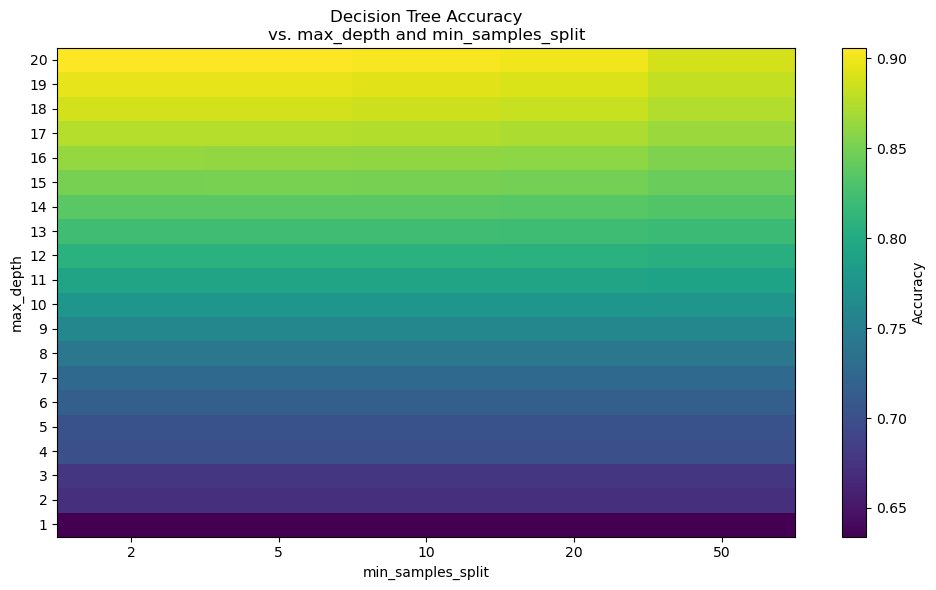
\includegraphics[width=1\linewidth]{../img/16}
	\caption{PID vs LMPC control effort RMSE}
	\label{fig:16}
\end{figure}
در نتیجه دیاگرام های سیستم ها با تجه به تغییرات اعمال شده به صورت زیر برای دو کنترلر خواهد بود.

\begin{figure}[H]
	\centering
	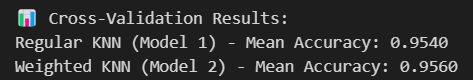
\includegraphics[width=1\linewidth]{../img/17}
	\caption{کنترلر Tube}
	\label{fig:17}
\end{figure}

\begin{figure}[H]
	\centering
	\includegraphics[width=1\linewidth]{../img/18}
	\caption{کنترلر LMPC}
	\label{fig:18}
\end{figure}

\subsection*{بخش دوم}
در این بخش، با افزودن یک کنترلر PID به MPC و تشکیل یک کنترلر $Tube MPC$، مجددا نتایج را بررسی می کنیم. بنابراین، ساختار سیستم طراحی شده به صورت زیر خواهد بود:

\begin{figure}[H]
	\centering
	\includegraphics[width=1\linewidth]{../img/19}
	\caption{کنترلر LMPC}
	\label{fig:19}
\end{figure}
در ادامه، با تنظیم مجدد کنترلر MPC و PID، کنترلر ها را مجددا طراحی می کنیم. تنظیم های کنترلر PID به صورت زیر خواهد بود.
\begin{figure}[H]
	\centering
	\includegraphics[width=1\linewidth]{../img/20}
	\caption{}
	\label{fig:20}
\end{figure}

\begin{figure}[H]
	\centering
	\includegraphics[width=1\linewidth]{../img/21}
	\caption{}
	\label{fig:21}
\end{figure}
تنظیمات MPC به صورت زیر خواهد بود:

\begin{figure}[H]
	\centering
	\includegraphics[width=1\linewidth]{../img/22}
	\caption{}
	\label{fig:22}
\end{figure}

% TODO: \usepackage{graphicx} required
\begin{figure}[h!]
	\centering
	\includegraphics[width=1\linewidth]{../img/23}
	\caption{}
	\label{fig:23}
\end{figure}

% TODO: \usepackage{graphicx} required
\begin{figure}[H]
	\centering
	\includegraphics[width=1\linewidth]{../img/24}
	\caption{}
	\label{fig:24}
\end{figure}

% TODO: \usepackage{graphicx} required
\begin{figure}[H]
	\centering
	\includegraphics[width=1\linewidth]{../img/25}
	\caption{}
	\label{fig:25}
\end{figure}

\newpage
\subsection*{بخش سوم}
در قسمت بعد، سیستم را با پیاده سازی کنترلر $Explicit MPC$ به جای کنترلر LMPC کنترل می کنیم. 
برای این کار با استفاده از دستورات $generateExplicitRange$،
$generateExplicitOptions$ و 
$generateExplicitMPC$
کنترلر MPC طراحی شده را با شرایط زیر به کنترلر EMPC تبدیل می کنیم. 
% TODO: \usepackage{graphicx} required
\begin{figure}[H]
	\centering
	\includegraphics[width=1\linewidth]{../img/26}
	\caption{}
	\label{fig:26}
\end{figure}

در اینجا لازم به ذکر است که استفاده از افق های پیش بینی و کنترل مورد استفاده در LMPC (افق پیش بین: 100، افق کنترل 30) برای کنترلر EMPC بسیار زیاد بوده و تعداد نواحی بسیار زیادی را ایجاد میکند که برای پیاده سازی، امکان پذیر نیست. بنابراین، پارامتر های این کنترلر به مقادیر زیر تغییر کرده اند.
افق پیش بین: 30
افق کنترل: 3

با اجرای برنامه، خروجی کنترلر به صورت زیر به دست می اید و مشاهده می شود که عملکردی مشابه با کنترلر LMPC دارد. 

\begin{figure}[H]
	\centering
	\includegraphics[width=0.7\linewidth]{../img/27}
	\caption{}
	\label{fig:27}
\end{figure}

مقادیر RMSE محاسبه شده برای این مدل به صورت زیر خواهد بود.
% TODO: \usepackage{graphicx} required
\begin{figure}[H]
	\centering
	\includegraphics[width=0.7\linewidth]{../img/28}
	\caption{ٍ}
	\label{fig:28}
\end{figure}

در نهایت، به مقایسه ی نتایج به دست آمده از کنترلر های ارائه شده برای این سیستم خواهیم پرداخت.

مقایسه حالت اول:
% TODO: \usepackage{graphicx} required
\begin{figure}[H]
	\centering
	\includegraphics[width=0.7\linewidth]{../img/29}
	\caption{}
	\label{fig:29}
\end{figure}

مقایسه حالت دوم:
% TODO: \usepackage{graphicx} required
\begin{figure}[H]
	\centering
	\includegraphics[width=0.7\linewidth]{../img/30}
	\caption{}
	\label{fig:30}
\end{figure}
مقایسه حالت سوم:
% TODO: \usepackage{graphicx} required
\begin{figure}[H]
	\centering
	\includegraphics[width=0.7\linewidth]{../img/31}
	\caption{}
	\label{fig:31}
\end{figure}
مقایسه تلاش کنترلی:
% TODO: \usepackage{graphicx} required
\begin{figure}[H]
	\centering
	\includegraphics[width=0.7\linewidth]{../img/32}
	\caption{}
	\label{fig:32}
\end{figure}


مقایسه RMSE حالت 1:
% TODO: \usepackage{graphicx} required
\begin{figure}[H]
	\centering
	\includegraphics[width=0.7\linewidth]{../img/33}
	\caption{}
	\label{fig:33}
\end{figure}

مقایسه RMSE حالت 3:
% TODO: \usepackage{graphicx} required
\begin{figure}[H]
	\centering
	\includegraphics[width=0.7\linewidth]{../img/34}
	\caption{}
	\label{fig:34}
\end{figure}

مقایسه RMSE کنترلر:
% TODO: \usepackage{graphicx} required
\begin{figure}[H]
	\centering
	\includegraphics[width=0.7\linewidth]{../img/35}
	\caption{}
	\label{fig:35}
\end{figure}

\subsection*{بخش چهارم}
در این بخش، یک کنترلر $Tube explicit MPC$ با اضافه کردن کنترلر PID به سیستم طراحی خواهد شد. ساختار دیاگرام این سیستم به صورت زیر است:
% TODO: \usepackage{graphicx} required
\begin{figure}[H]
	\centering
	\includegraphics[width=0.7\linewidth]{../img/36}
	\caption{}
	\label{fig:36}
\end{figure}

ضرایب PID مانند کنترلر $Tube MPC$ طراحی شده است و بلوک EMPC نیز با استفاده از تنظیمات نمایش داده شده در بخش قبل در دیاگرام قرار گرفته است.
پاسخ های به دست آمده از این سیستم در شکل زیر نمایش داده شده است.
% TODO: \usepackage{graphicx} required
\begin{figure}[H]
	\centering
	\includegraphics[width=0.7\linewidth]{../img/37}
	\caption{}
	\label{fig:37}
\end{figure}

همچنین نمودار تلاش کنترلی این سیستم به صورت زیر است:
% TODO: \usepackage{graphicx} required
\begin{figure}[H]
	\centering
	\includegraphics[width=0.7\linewidth]{../img/38}
	\caption{}
	\label{fig:38}
\end{figure}

و مقادیر RMSE به دست آمده برای این سیستم در شکل زیر نمایش داده شده است:
% TODO: \usepackage{graphicx} required
\begin{figure}[H]
	\centering
	\includegraphics[width=0.7\linewidth]{../img/39}
	\caption{}
	\label{fig:39}
\end{figure}
% TODO: \usepackage{graphicx} required
\begin{figure}[H]
	\centering
	\includegraphics[width=0.7\linewidth]{../img/40}
	\caption{}
	\label{fig:40}
\end{figure}

در پایان این بخش، به مقایسه ی نتایج به دست آمده از کنترلر TEMPC با کنترلر TMPC خواهیم پرداخت.
نمودار خروجی حالت اول سیستم با استفاده از این دو کنترلر به صورت زیر است:
% TODO: \usepackage{graphicx} required
\begin{figure}[H]
	\centering
	\includegraphics[width=0.7\linewidth]{../img/41}
	\caption{}
	\label{fig:41}
\end{figure}

همچنین، نمودار تلاش کنترلی برای این دو در شکل زیر نمایش داده شده است:
% TODO: \usepackage{graphicx} required
\begin{figure}[H]
	\centering
	\includegraphics[width=0.7\linewidth]{../img/42}
	\caption{}
	\label{fig:42}
\end{figure}

در نهایت، مقادیر RMSE به دست آمده برای این دو کنترلر به صورت زیر است:
% TODO: \usepackage{graphicx} required
\begin{figure}[H]
	\centering
	\includegraphics[width=0.7\linewidth]{../img/43}
	\caption{}
	\label{fig:43}
\end{figure}
% TODO: \usepackage{graphicx} required
\begin{figure}[H]
	\centering
	\includegraphics[width=0.7\linewidth]{../img/44}
	\caption{}
	\label{fig:44}
\end{figure}
% TODO: \usepackage{graphicx} required
\begin{figure}[H]
	\centering
	\includegraphics[width=0.7\linewidth]{../img/45}
	\caption{}
	\label{fig:45}
\end{figure}
\section{پاسخ سوال دو}
برای طراحی کنترلر $Hybrid MPC$، برای سیستمم ارائه شده، لازم است تا با استفاده از یک سوییچ، تو بلوک حالت سیستم را به صورت موازی در سیستم قرار داده و سپس با طراحی یک ماشین حالت، جابه جایی میان آن دو را ممکن ساخت. بنابراین، دیاگرام سیستم به صورت زیر تشکیل می شود.
% TODO: \usepackage{graphicx} required
\begin{figure}
	\centering
	\includegraphics[width=0.7\linewidth]{../img/47}
	\caption{دیاگرام کنترلر هیبرید}
	\label{fig:47}
\end{figure}
با قرار دادن شرط سوییچ برای ماشین حالت به صورتی که اگر مقدار خروجی کمتر از -5 باشد، در مد اول و اگر بیشتر از 5 باشد در مد کاری دوم باشد، معین می شود.
سپس، با طراحی کنترلر MPC با افق پیش بین 110 و افق کنترلی 8 سیستم کنترل می شود. لازم به ذکر است که در این بخش، قید های خواسته شده توسط سوال برای مقادیر ورودی بازه ی $-30$ و $30$ در نظر گرفته شده است. 
با اجرای سیستم، خروجی های کنترلر، مقدار رفرنس و خروجی سیستم به صورت زیر به دست می آیند و مشاهده می شود که کنترلر توانسته است به خوبی خروجی را کنترل کند. اگرچه، در نقطه ی تغییر مد سیستم، نوسانی مشاهده می شود که با تلاش کنترلی، به راحتی حذف شده است.
% TODO: \usepackage{graphicx} required
\begin{figure}
	\centering
	\includegraphics[width=0.7\linewidth]{../img/46}
	\caption{}
	\label{fig:46}
\end{figure}






















		% فصل چهارم: نتایج
%\include{./tex/chapter5}		% فصل پنجم: بحث و نتیجه‌گیری

% مراجع
% اگر از استیل‌های natbib استفاده می‌کنید باید دو خط را در فایل commands.tex تغییر دهید.
%\pagestyle{empty}
%\newpage
%{
%\small
%\onehalfspacing
%\bibliographystyle{unsrt-fa} % or plainnat-fa for author-date
%\bibliography{./tex/MyReferences}
%}

\pagestyle{fancy}

%\appendix
% فصلهای پس از این قسمت به عنوان ضمیمه خواهند آمد.

% دستورات لازم برای تبدیل «فصل آ» به «پیوست آ» در فهرست مطالب

%\addtocontents{toc}{
%\protect\renewcommand\protect\cftchappresnum{\appendixname~}%
%\protect\setlength{\cftchapnumwidth}{\mylenapp}}
    
% دستورات لازم برای شماره‌گذاری صفحات پیوست‌ها بشکل آ-۱ (فعلا با glossaries سازگار نیست)
%\let\Chapter\chapter
%\pretocmd{\chapter}{
%\clearpage
%\pagenumbering{arabic}
%\renewcommand*{\thepage}{\rl{\thechapter-\arabic{page}}}}{}{}
%%%%%%%%%%%%%%%%%%%%%%%%%%%%%%%%%%%%%        

%\include{./tex/appendix1}		% پیوست اول: آشنایی مقدماتی با لاتک
%\include{./tex/appendix2}		% پیوست دوم: جدول، نمودار و الگوریتم در لاتک
%\include{./tex/appendix3}   	% پیوست سوم: مراجع، واژه‌نامه و حاشیه‌نویسی

%\onehalfspacing
%\cleardoublepage
% برگرداندن شماره‌بندی صفحات فصول
\let\chapter\Chapter
\pagenumbering{tartibi} % اول، دوم، ...
\baselineskip=.75cm

% چاپ واژه‌نامه‌ها و نمایه: در صورتی که نمی‌خواهید واژه‌نامه‌ها و نمایه نمایش داده شوند سه خط زیر را کامنت نمایید.
%\printglossary
%\cleardoublepage
%\printindex

%\begin{latin}
%\baselineskip=.6cm
%\latinabstract
%\latinTitlePage
%\end{latin}
%\label{LastPage}

\end{document}
